\documentclass[extra,mreferee]{gji}
%DIF LATEXDIFF DIFFERENCE FILE
%DIF DEL original.tex   Wed Nov  8 20:59:31 2017
%DIF ADD new.tex        Wed Nov  8 20:59:53 2017
%\documentclass[extra,onecolumn,doublespacing]{gji}
\usepackage{timet}
\usepackage{amsmath}
\usepackage{amsfonts}
\usepackage{amssymb}
\usepackage{graphicx}
\usepackage{arydshln}
\usepackage{bm}
\usepackage{ulem}

\title[Transient strain in geodetic data]
      {Revealing transient strain in geodetic data with Gaussian process regression}

\author[T. T. Hines and E. A. Hetland]
       {T. T. Hines$^1$ and E. A. Hetland$^1$ \\
        $^1$ Department of Earth and Environmental Sciences, University of Michigan, Ann Arbor, MI, USA}

\date{Received XXX; in original form XXX}

\pagerange{\pageref{firstpage}--\pageref{lastpage}}

\volume{XXX}

\pubyear{XXX}

% Authors with AMS fonts and mssymb.tex can comment out the following
% line to get the correct symbol for Geophysical Journal International.
\let\leqslant=\leq

\newtheorem{theorem}{Theorem}[section]
%DIF PREAMBLE EXTENSION ADDED BY LATEXDIFF
%DIF UNDERLINE PREAMBLE %DIF PREAMBLE
\RequirePackage[normalem]{ulem} %DIF PREAMBLE
\RequirePackage{color}\definecolor{RED}{rgb}{1,0,0}\definecolor{BLUE}{rgb}{0,0,1} %DIF PREAMBLE
\providecommand{\DIFadd}[1]{{\protect\color{blue}\uwave{#1}}} %DIF PREAMBLE
\providecommand{\DIFdel}[1]{{\protect\color{red}\sout{#1}}}                      %DIF PREAMBLE
%DIF SAFE PREAMBLE %DIF PREAMBLE
\providecommand{\DIFaddbegin}{} %DIF PREAMBLE
\providecommand{\DIFaddend}{} %DIF PREAMBLE
\providecommand{\DIFdelbegin}{} %DIF PREAMBLE
\providecommand{\DIFdelend}{} %DIF PREAMBLE
%DIF FLOATSAFE PREAMBLE %DIF PREAMBLE
\providecommand{\DIFaddFL}[1]{\DIFadd{#1}} %DIF PREAMBLE
\providecommand{\DIFdelFL}[1]{\DIFdel{#1}} %DIF PREAMBLE
\providecommand{\DIFaddbeginFL}{} %DIF PREAMBLE
\providecommand{\DIFaddendFL}{} %DIF PREAMBLE
\providecommand{\DIFdelbeginFL}{} %DIF PREAMBLE
\providecommand{\DIFdelendFL}{} %DIF PREAMBLE
%DIF END PREAMBLE EXTENSION ADDED BY LATEXDIFF

\begin{document}

\label{firstpage}

\maketitle

%DIF > % DEFINE MATH MODE MACROS
%DIF > %%%%%%%%%%%%%%%%%%%%%%%%%%%%%%%%%%%%%%%%%%%%%%%%%%%%%%%%%%%%%%%%%%%%
\DIFaddbegin \newcommand{\pos}{\vec{x}} %DIF >  position vector
\newcommand{\data}{\mitbf{d}} %DIF >  data vector
\newcommand{\post}{\hat{u}} %DIF >  posterior
\newcommand{\points}{\mitbf{P}} %DIF >  observation points
\newcommand{\strain}{\dot\varepsilon} %DIF >  strain rate
\newcommand{\E}[1]{\mathrm{E}\left[ #1 \right]} %DIF >  Expected value
\newcommand{\Cov}[1]{\mathrm{Cov}\left[ #1 \right]} %DIF >  Expected value
\newcommand{\e}{\mathrm{e}} %DIF >  east subscript
\newcommand{\n}{\mathrm{n}} %DIF >  north subscript
\newcommand{\G}{\mitbf{G}} %DIF >  basis functions
\newcommand{\zeros}{\mitbf{0}} %DIF >  zeros matrix
\newcommand{\eye}{\mitbf{I}} %DIF >  identity matrix

%DIF > % SUMMARY
%DIF > %%%%%%%%%%%%%%%%%%%%%%%%%%%%%%%%%%%%%%%%%%%%%%%%%%%%%%%%%%%%%%%%%%%%
\DIFaddend \begin{summary}
\DIFaddbegin 

%DIF >  focus on subjective vs object rather than "we have uncertainties"

\DIFaddend Transient strain rates derived from GNSS data can be used to detect
and understand geophysical \DIFdelbegin \DIFdel{phenomena }\DIFdelend \DIFaddbegin \DIFadd{processes }\DIFaddend such as slow slip events and
postseismic deformation. Here we propose using Gaussian process
regression (GPR) as a tool for estimating transient strain rates from
GNSS data. GPR is a non-parametric, Bayesian method for interpolating
scattered data. \DIFdelbegin \DIFdel{Transient strain rates estimated with GPR have meaningful uncertainties, allowing geophysical signal to be easily discerned from noise. }\DIFdelend In our approach, we assume a stochastic prior model
for transient displacements. The prior describes how much \DIFdelbegin \DIFdel{one expects }\DIFdelend \DIFaddbegin \DIFadd{we expect
}\DIFaddend transient displacements to covary spatially and temporally. A
posterior estimate of transient strain rates is obtained by
differentiating the posterior displacements\DIFdelbegin \DIFdel{. One limitation with GPR is that it is not robust against outliers, so we introduce a pre-processing method for detecting and removing outliers in }\DIFdelend \DIFaddbegin \DIFadd{, which are formed by
conditioning the prior with the }\DIFaddend GNSS data. As a demonstration, we use
GPR to detect transient strain resulting from slow slip events in \DIFdelbegin \DIFdel{Cascadia}\DIFdelend \DIFaddbegin \DIFadd{the
Pacific Northwest}\DIFaddend . Maximum likelihood methods are used to constrain a
prior model for transient displacements in this region. The temporal
covariance of our prior model is described by a compact Wendland
covariance function, which significantly reduces the computational
burden that can be associated with GPR. Our results reveal the spatial
and temporal evolution of strain from slow slip events. We verify that
the transient strain estimated with GPR is in fact geophysical signal
by comparing it to the seismic tremor that is associated with \DIFdelbegin \DIFdel{Cascadia }\DIFdelend \DIFaddbegin \DIFadd{Pacific
Northwest }\DIFaddend slow slip events.
\DIFaddbegin 

\DIFaddend \end{summary}

\begin{keywords}
 XXX -- XXX -- XXX -- XXX.
\end{keywords}

%DIF > % INTRODUCTION
%DIF > %%%%%%%%%%%%%%%%%%%%%%%%%%%%%%%%%%%%%%%%%%%%%%%%%%%%%%%%%%%%%%%%%%%%
\section{Introduction}\label{sec:Introduction}
\DIFaddbegin 

%DIF >  Why we care about determining strain

\DIFaddend Crustal strain rates are fundamentally important quantities for
assessing seismic hazard. Knowing where and how quickly strain is
accumulating gives insight into where we can expect stored elastic
energy to be released seismically. Consequently, secular crustal
strain rates estimated from GNSS data have been used to constrain
seismic hazard models such as UCERF3 \citep{Field2014}. Transient
crustal strain, which is caused by geophysical phenomena such as slow
slip events (SSEs) or postseismic deformation, is also relevant for
assessing seismic hazard. While transient strain itself is not
damaging, there is a risk that it can trigger major earthquakes
\citep{Roeloffs2006,Freed2001}. Dense networks of continuous GNSS
stations, such as the Plate Boundary Observatory (PBO), make it
possible to identify transient strain with high fidelity. Developing
and improving upon methods for deriving secular and transient strain
from GNSS data is an active area of research.

%DIF >  Existing methods for determining secular strain from GPS
\DIFaddbegin 

\DIFaddend Most methods for estimating strain rates from GNSS data assume some
parametric form \DIFdelbegin \DIFdel{of }\DIFdelend \DIFaddbegin \DIFadd{for }\DIFaddend the deformation signal. The simplest method for
estimating secular strain rates assumes that GNSS derived velocities
can be described with a first-order polynomial (i.e\DIFdelbegin \DIFdel{., having constant deformation
gradients }\DIFdelend \DIFaddbegin \DIFadd{, the deformation
gradients are constant}\DIFaddend ) over some subnetwork of the GNSS stations
\citep[e.g.,][]{Feigl1990,Murray2000}. The components of the strain
rate tensor for each subnetwork are then determined \DIFdelbegin \DIFdel{through a }\DIFdelend \DIFaddbegin \DIFadd{from the }\DIFaddend least
squares fit to the observations. The assumption that deformation
gradients are spatially uniform is not appropriate when subnetworks
span too large of an area. To help overcome this deficiency,
\citet{Shen1996,Shen2015} used an inverse distance weighting scheme,
in which the estimated strain rate at \DIFdelbegin \DIFdel{some }\DIFdelend \DIFaddbegin \DIFadd{a }\DIFaddend point is primarily controlled
by observations at nearby stations. \DIFdelbegin \DIFdel{However, the methods described in \mbox{%DIFAUXCMD
\citet{Shen1996,Shen2015} }%DIFAUXCMD
are still formulated by assuming that the deformation gradients are uniform over the entire network. The errors in this assumption manifest as implausibly low formal uncertainties for the estimated strain rates}\DIFdelend \DIFaddbegin \DIFadd{The method of
\mbox{%DIFAUXCMD
\citet{Shen1996,Shen2015} }%DIFAUXCMD
can be viewed as a form of local least
squares regression with a first-order polynomial \mbox{%DIFAUXCMD
\citep[e.g.,][sec.
6]{Hastie2009}}%DIFAUXCMD
}\DIFaddend . Other methods for estimating secular strain rates have
parameterized GNSS derived velocities with bi-cubic splines
\citep{Beavan2001}, spherical wavelets \citep{Tape2009}, and
elastostatic Green's functions \citep{Sandwell2016}. The type of basis
functions and the number of degrees of freedom for a parameterization\DIFdelbegin \DIFdel{can be subjective}\DIFdelend \DIFaddbegin \DIFadd{,
which are often chosen subjectively, have a strong influence on the
strain solution}\DIFaddend . If there are too few degrees of freedom in the
parameterization, then estimated strain rates will be biased and the
uncertainties will be underestimated. On the other hand, if there are
too many degrees of freedom, then there will not be any coherent
features in the estimated strain rates. The methods described by
\citet{Beavan2001} and \citet{Tape2009} also require the user to
specify penalty parameters that control a similar trade-off between
bias and variance in the solution. One could parameterize deformation
with a physically motivated model of interseismic deformation
\citep[e.g.,][]{Meade2005,McCaffrey2007}. In such models the
lithospheric rheology and fault geometries are assumed to be known.
Any errors in the assumed physical model could result in biased strain
estimates and underestimated formal uncertainties.

%DIF >  Existing methods for determining transient strain from GPS
\DIFaddbegin 

\DIFaddend The aforementioned studies are concerned with estimating secular
strain rates. In recent years the Southern California Earthquake
Center (SCEC) community has shown interest in developing methods for
detecting transient strain. SCEC supported a transient detection
exercise \citep{Lohman2013}, where several research groups tested
their methods for detecting transient geophysical signal with a
synthetic GNSS dataset. Among the methods tested were the Network
Strain Filter (NSF) \citep{Ohtani2010} and the Network Inversion
Filter (NIF) \citep{Segall1997}. The NSF uses a wavelet
parameterization to describe the spatial component of geophysical
signal. The NIF, which is intended for imaging slow fault slip from
geodetic data, uses the elastic dislocation Green's functions from
\citet{Okada1992}. For the NSF and NIF, the time dependence of the
geophysical signal is modeled as integrated Brownian motion. The
method described in \citet{Holt2013} was also tested in the SCEC
transient detection exercise, which calculates strain rates using a
bi-cubic spatial parameterization of displacements between time
epochs. \citet{Holt2013} defined a detection threshold based on the
strain rate magnitude, and \DIFdelbegin \DIFdel{below }\DIFdelend we demonstrate that this is indeed an
effective criterion for identifying geophysical signal. For the same
reasons descibed above, the transient deformation and corresponding
uncertainties estimated by these methods can be biased by the chosen
spatial parameterization. It is then difficult to distinguish signal
from noise with these methods, which limits their utility for
transient detection.

%DIF >  What we are doing in this paper and why it improves upon existing
%DIF >  methods
\DIFaddbegin 

\DIFaddend Here we propose using Gaussian process regression (GPR)
\citep{Rasmussen2006} to estimate transient strain from GNSS data. GPR
is \DIFaddbegin \DIFadd{closely related to kriging \mbox{%DIFAUXCMD
\citep{Cressie1992} }%DIFAUXCMD
and least squares
collocation \mbox{%DIFAUXCMD
\citep{Moritz1978}}%DIFAUXCMD
. The latter has been used by
\mbox{%DIFAUXCMD
\citet{Kato1998} }%DIFAUXCMD
and \mbox{%DIFAUXCMD
\citet{El-Fiky1999} }%DIFAUXCMD
to estimate secular strain
rates from GNSS data. GPR is }\DIFaddend a Bayesian, non-parametric method for
inferring a continuous signal from scattered data. Since GNSS stations
are irregularly spaced and observation times may differ between
stations, GPR is an ideal tool for synthesizing \DIFaddbegin \DIFadd{discrete }\DIFaddend GNSS data
into a spatially and temporally continuous representation of \DIFdelbegin \DIFdel{surface deformation. GPR is closely related to kriging \mbox{%DIFAUXCMD
\citep{Cressie1992} }%DIFAUXCMD
and least squares collocation \mbox{%DIFAUXCMD
\citep{Moritz1978}}%DIFAUXCMD
. The latter has been used by \mbox{%DIFAUXCMD
\citet{Kato1998} }%DIFAUXCMD
and \mbox{%DIFAUXCMD
\citet{El-Fiky1999} }%DIFAUXCMD
to estimate secular strainrates from GNSS data}\DIFdelend \DIFaddbegin \DIFadd{transient
strain}\DIFaddend . GPR is Bayesian in that we \DIFdelbegin \DIFdel{describe our prior understanding of the geophysical signal with a Gaussian process. A Gaussian process is a normally distributed stochastic processthat is fully defined in terms of a mean function and a positive-definite covariance function. For example, Brownian motion, $B(t)$, is a well known Gaussian processin $\mathbb{R}^1$ which has zero mean and covariance function $\mathrm{cov}(B(t),B(t')) = \min(t,t')$, where $t,t' \ge 0$.
If no prior information is available for the geophysical signal}\DIFdelend \DIFaddbegin \DIFadd{use a prior model to control the
spatial and temporal roughness of the inferred transient strain. The
prior is specified as a stochastic process, namely a Gaussian process.
If there is no information available to help choose an appropriate
prior Gaussian process}\DIFaddend , then maximum likelihood methods can be used to
\DIFdelbegin \DIFdel{choose a prior Gaussian process }\DIFdelend \DIFaddbegin \DIFadd{objectively choose one }\DIFaddend that is most consistent with the \DIFdelbegin \DIFdel{observations.  We incorporate GNSS observations with the prior to form a posterior estimate of transient strain.  The posterior transient strain is also a Gaussian process, and we can use its distribution to confidently discern geophysical signal from noise}\DIFdelend \DIFaddbegin \DIFadd{data}\DIFaddend . We use
GPR to infer transient strain resulting from SSEs in \DIFdelbegin \DIFdel{Cascadia. Our results demonstrate }\DIFdelend \DIFaddbegin \DIFadd{the Pacific
Northwest, demonstrating }\DIFaddend that GPR is an effective tool for detecting
\DIFdelbegin \DIFdel{SSEs and revealing how strain evolves during SSEs}\DIFdelend \DIFaddbegin \DIFadd{transient geophysical processes}\DIFaddend .


%DIF > % ESTIMATING TRANSIENT STRAIN RATES
%DIF > %%%%%%%%%%%%%%%%%%%%%%%%%%%%%%%%%%%%%%%%%%%%%%%%%%%%%%%%%%%%%%%%%%%%
\section{Estimating Transient Strain Rates}\label{sec:Method}
\DIFaddbegin 

%DIF >  Overview of what we are trying to do in this section and how

\DIFaddend We seek a spatially and temporally dependent estimate of transient
\DIFdelbegin \DIFdel{crustal }\DIFdelend strain rates. We consider transient strain rates to be any deviation
from \DIFaddbegin \DIFadd{the }\DIFaddend secular strain rates\DIFdelbegin \DIFdel{, and our attention is limited to horizontal strain rates in this study}\DIFdelend . We denote transient \DIFdelbegin \DIFdel{crustal }\DIFdelend strain rates as
\DIFdelbegin \DIFdel{$\dot\varepsilon(p)$}\DIFdelend \DIFaddbegin \DIFadd{$\strain(p)$}\DIFaddend , where $p$ represents the ordered pair \DIFdelbegin \DIFdel{$(\vec{x},t)$, $\vec{x}$ }\DIFdelend \DIFaddbegin \DIFadd{$(\pos,t)$, $\pos
= (x_\e,x_\n)$ }\DIFaddend are spatial coordinates\DIFdelbegin \DIFdel{in $\mathbb{R}^2$}\DIFdelend , and $t$ is time. \DIFdelbegin \DIFdel{We determine $\dot\varepsilon(p)$ }\DIFdelend \DIFaddbegin \DIFadd{The
subscripts ``e" and ``n" indicate the east and north component, and we
assume that the study region is sufficiently small that $\pos$ can be
considered a point in a 2-D Cartesian map projection that is aligned
with the cardinal directions. We determine $\strain$ }\DIFaddend by spatially and
temporally differentiating estimates of transient displacements, \DIFdelbegin \DIFdel{$\vec{u}(p)$.
We make a prior assumption that }\DIFdelend \DIFaddbegin \DIFadd{which
we constrain with GNSS data.
}

%DIF >  Defining u as a prior Gaussian process

\DIFadd{We let $\vec{u}(p) = (u_\e(p),u_\n(p))$ be our prior understanding of
transient displacements. Since transient displacements are not
precisely known, we cannot consider $\vec{u}$ to be a deterministic
function. Instead, $\vec{u}$ is considered to be a stochastic process
containing a distribution of functions that could potentially describe
transient displacements. Specifically, we let }\DIFaddend each component of
$\vec{u}$ \DIFdelbegin \DIFdel{is }\DIFdelend \DIFaddbegin \DIFadd{be }\DIFaddend a Gaussian process\DIFdelbegin \DIFdel{,
}\begin{displaymath}\DIFdel{%DIFDELCMD < \label{eq:TransientDeformation}%%%
u_i(p) \sim \mathcal{N}\left(0,C_{u_i}\right),
}\end{displaymath}
%DIFAUXCMD
\DIFdel{where $C_{u_i}(p,p')$ is }\DIFdelend \DIFaddbegin \DIFadd{. A Gaussian process is a stochastic
process whose value at any collection of points can be described with
a multivariate normal distribution. That is to say, the random vector
$[u_i(p)]_{p \in \points}$ has a multivariate normal distribution for
any collection of points $\points$. A realization of the random vector
$[u_i(p)]_{p \in \points}$ can be interpretted as a realization of
$u_i$ (i.e., a sample function) that is evaluated at $\points$. Just
as a multivariate normal distribution is fully determined by a mean
vector and a covariance matrix, a Gaussian process is fully determined
by a mean function and }\DIFaddend a covariance function\DIFdelbegin \DIFdel{indicating how we expect $u_i(p)$ to covary with $u_i(p')$. For simplicity, we treat }\DIFdelend \DIFaddbegin \DIFadd{. For example, Brownian
motion, $B(t)$, is a well known Gaussian process in $\mathbb{R}^1$
which has the mean function $\E{B(t)} = 0$ and the covariance function
$\Cov{B(t),B(t')} = \min(t,t')$, where $t,t' \ge 0$. We let }\DIFaddend each
component of \DIFdelbegin \DIFdel{displacements independently and ignore any potential covariance
. Hence, we drop the component subscripts with the understanding that the same analysis is being repeated to estimate the easting and northing components of }\DIFdelend $\vec{u}$ \DIFaddbegin \DIFadd{have zero mean and a generic covariance
function $\Cov{u_i(p),u_i(p')} = C_{u_i}(p,p')$. Using a more concise
notation, we write our prior on each component of $\vec{u}$ as $u_i
\sim \mathcal{GP}\left(0,C_{u_i}\right)$.
}

%DIF >  Constraints on the Covariance function

\DIFadd{The function $C_{u_i}$ must be positive definite in order to be a
valid covariance function. By definition, $C_{u_i}$ is a positive
definite function if the matrix $[C_{u_i}(p,p')]_{(p,p') \in \points
\times \points}$ is positive definite for any set of points $\points$
\mbox{%DIFAUXCMD
\citep[sec. 2.5]{Cressie1992}}%DIFAUXCMD
}\DIFaddend . We assume that \DIFdelbegin \DIFdel{$C_u$ }\DIFdelend \DIFaddbegin \DIFadd{$C_{u_i}$ }\DIFaddend can be
separated into \DIFdelbegin \DIFdel{positive definite }\DIFdelend spatial and temporal functions as
\begin{equation}\label{eq:TransientCovariance}
C\DIFdelbegin \DIFdel{_{u}}\DIFdelend \DIFaddbegin \DIFadd{_{u_i}(p,p') = C_{u_i}}\DIFaddend \left((\DIFdelbegin %DIFDELCMD < \vec{x}%%%
\DIFdelend \DIFaddbegin \pos\DIFaddend ,t),(\DIFdelbegin %DIFDELCMD < \vec{x}%%%
\DIFdelend \DIFaddbegin \pos\DIFaddend ',t')\right) 
              = X\DIFaddbegin \DIFadd{_i}\DIFaddend (\DIFdelbegin %DIFDELCMD < \vec{x}%%%
\DIFdelend \DIFaddbegin \pos\DIFaddend ,\DIFdelbegin %DIFDELCMD < \vec{x}%%%
\DIFdelend \DIFaddbegin \pos\DIFaddend ')T\DIFaddbegin \DIFadd{_i}\DIFaddend (t,t').
\end{equation}   
\DIFaddbegin \DIFadd{As long as the functions $X_i$ and $T_i$ are positive definite,
$C_{u_i}$ is guaranteed to also be positive definite \mbox{%DIFAUXCMD
\citep[sec.
4.2.4]{Rasmussen2006}}%DIFAUXCMD
. We also require that the derivatives
$\partial^2 X_i(\pos,\pos')/ \partial x_j \partial x_j'$ and
$\partial^2 T_i(t,t') / \partial t \partial t'$ exist. This ensures
that $u_i$ is spatially and temporally differentiable, allowing us to
compute transient strain rates (See \mbox{%DIFAUXCMD
\citet[sec. 2.2]{Adler1981} }%DIFAUXCMD
or
\mbox{%DIFAUXCMD
\citet[sec. 10A]{Papoulis1991} }%DIFAUXCMD
for a definition of stochastic
differentiation and the conditions for differentiability).
}

%DIF >  Example of the prior

\DIFadd{We provide an example to give the prior on transient displacements a
more tangible meaning. we can use a squared exponential function for
$X_i$ and $T_i$,
}\begin{equation}\DIFadd{\label{eq:ExampleCov}
X_i(\pos,\pos') = \exp\left(\frac{-||\pos - \pos'||_2^2}{2\ell^2}\right), \ \ \ \ 
T_i(t,t') = \phi^2 \exp\left(\frac{-|t - t'|^2}{2\tau^2}\right),
}\end{equation}
\DIFadd{which satisfies our requirements for positive definiteness and
differentiability. The parameters $\ell$ and $\tau$ control the
length-scale and time-scale, respectively, of realizations of $u_i$.
The parameter $\phi$, which we have arbitrarily chosen to incorporate
into $T_i$ rather than $X_i$, controls the amplitude of realizations
of $u_i$. Ideally, we want realizations of $u_i$ to have a
length-scale, time-scale, and amplitude that resemble what we expect
for the true transient displacements. In Figure \ref{fig:PriorDemo}A,
we show $C_{u_i}$ using the squared exponential function for $X_i$ and
$T_i$ and the parameters $\ell = 100$ km, $\tau = 10$ days, and $\phi
= 1$ mm. A single realization of $u_i$ corresponsing to that choice of
covariance function is shown in Figure \ref{fig:PriorDemo}B (See
\mbox{%DIFAUXCMD
\citet[sec. A3]{Rasmussen2006} }%DIFAUXCMD
for details on drawing realization from
Gaussian processes). While the squared exponential function is a
commonly used covariance function for GPR, it is not appropriate for
every application. }\DIFaddend The appropriate choice for \DIFdelbegin \DIFdel{$X$ and $T$ }\DIFdelend \DIFaddbegin \DIFadd{$X_i$ and $T_i$ }\DIFaddend may vary
depending on the geophysical signal we are trying to describe\DIFdelbegin \DIFdel{, and we discuss this matter in Section \ref{sec:SignalModel}}\DIFdelend \DIFaddbegin \DIFadd{. To keep
this section sufficiently general, we hold off on specifying $X_i$ and
$T_i$ until Section \ref{sec:SignalModel}, where we estimate transient
strain from slow slip events in the Pacific Northwest}\DIFaddend .

\DIFdelbegin \DIFdel{We constrain $u$ with GNSS data , which records $u$ }\DIFdelend \DIFaddbegin \begin{figure*}
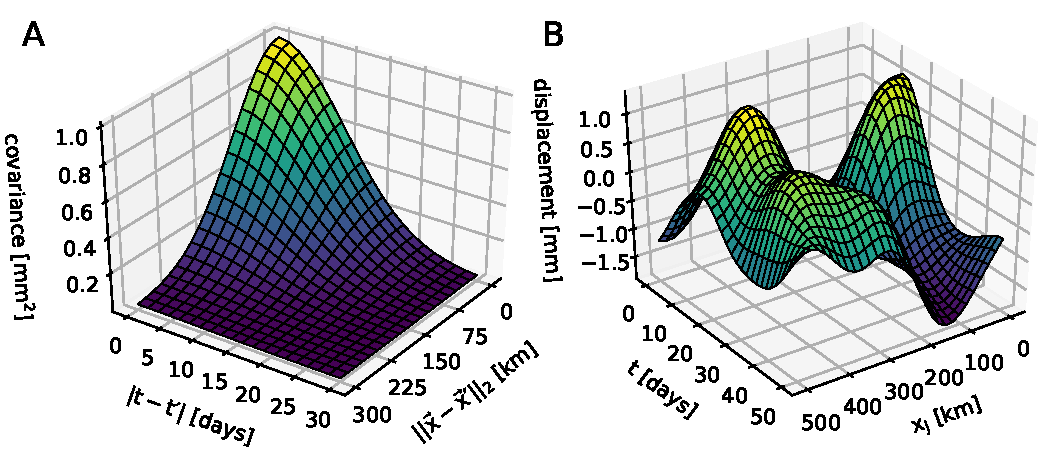
\includegraphics{figures/prior_demo/prior-demo.pdf}
\caption{ 
\DIFaddFL{(A) An example covariance function for transient displacements,
$C_{u_i}(p,p')$, shown as a function of the spatial and temporal
distance between $p$ and $p'$. (B) A single realization of transient
displacements, $u_i(p)$, corresponding to the covariance function from
Panel A. The realization is a function of three variables, $t$,
$x_\mathrm{e}$, and $x_\mathrm{n}$, although we only show its
dependence on $t$ and one of the spatial dimensions.
}}    
\label{fig:PriorDemo}
\end{figure*}

%DIF >  define the components of a datum 

\DIFadd{GNSS data records transient displacements }\DIFaddend as well as other physical
and non-physical processes that we are not interested in. We \DIFdelbegin \DIFdel{describe GNSS observations at position $\vec{x}_i$ and time $t_j$ }\DIFdelend \DIFaddbegin \DIFadd{first
consider component $i$ of a single GNSS displacement observation made
at station $j$, which is located at $\pos^{(j)}$, and time $t^{(k)}$.
We describe this observation, $d_i^{*(jk)}$, }\DIFaddend as a realization of the
random variable
\begin{align}\label{eq:Data}
\DIFdelbegin %DIFDELCMD < \begin{split}
%DIFDELCMD < d_{ij} = &u(\vec{x}_i,t_j) + \eta(\vec{x}_i,t_j) + w_{ij} + a^{(1)}_i + a^{(2)}_it_j + \\
%DIFDELCMD <          &a^{(3)}_i\sin(2 \pi t_j) + a^{(4)}_i\cos(2 \pi t_j) + a^{(5)}_i\sin(4 \pi t_j) + a^{(6)}_i\cos(4 \pi t_j), 
%DIFDELCMD < \end{split}
%DIFDELCMD < %%%
\DIFdelend \DIFaddbegin \begin{split}
d_i^{(jk)} = &u_i\left(\pos^{(j)},t^{(k)}\right) + 
              \eta_i^{(jk)} + 
              a_i^{(j)} + b_i^{(j)}t^{(k)} + \\
             &c_i^{(j)}\sin\left(2 \pi t^{(k)}\right) +  
              e_i^{(j)}\cos\left(2 \pi t^{(k)}\right) + \\ 
             &f_i^{(j)}\sin\left(4 \pi t^{(k)}\right)  + 
              g_i^{(j)}\cos\left(4 \pi t^{(k)}\right), 
\end{split}
\DIFaddend \end{align}
where \DIFdelbegin \DIFdel{$a^{(1)}_{i}$ }\DIFdelend \DIFaddbegin \DIFadd{$\eta_i^{(jk)}$ describes noise, $a_i^{(j)}$ }\DIFaddend is an offset that
is unique for each \DIFdelbegin \DIFdel{GNSS monument, $a^{(2)}_{i}$ }\DIFdelend \DIFaddbegin \DIFadd{station, $b_i^{(j)}$ }\DIFaddend is the secular velocity at
\DIFdelbegin \DIFdel{$\vec{x}_i$}\DIFdelend \DIFaddbegin \DIFadd{$\pos^{(j)}$}\DIFaddend , and the sinusoids describe seasonal deformation (using
units of years for \DIFdelbegin \DIFdel{$t_j$). 
We use $w_{ij}$ to denote normally distributed, uncorrelated noise. Correlated noise which does not have a parametric representation is denoted by $\eta$. For example, $\eta$ can consist of temporally correlated noise describing benchmark wobble \mbox{%DIFAUXCMD
\citep[e.g.,][]{Wyatt1982,Wyatt1989}}%DIFAUXCMD
, and/or spatially correlated noise describing common mode error \mbox{%DIFAUXCMD
\citep[e.g.,][]{Wdowinski1997}}%DIFAUXCMD
. For now, we will only assume that $\eta \sim \mathcal{N}(0,C_\eta)$. We consider the six coefficients in }\DIFdelend \DIFaddbegin \DIFadd{$t^{(k)}$). 
}

%DIF >  define the data vector 

\DIFadd{We then consider the column vector of $n$ GNSS displacement
observations, $\data^*_i$, where the subscript indicates that we are
still only considering component $i$ of displacements. The
observations are made at $m$ stations, and the times and positions for
each observation are described by the set $\points$. The data vector
$\data^*_i$ can be considered a realization of the random vector
$\data_i$, which is formed by evaluating eq. (\ref{eq:Data}) at each
point in $\points$. To write out $\data_i$ explicitly, we let $\G$ be
an $n \times 6m$ matrix consisting of the basis functions from }\DIFaddend eq.
(\ref{eq:Data}) \DIFdelbegin \DIFdel{to be uncorrelated random variables distributed as $\mathcal{N}(0,\kappa^2)$ in the limit as $\kappa \to \infty$ }\DIFdelend (i.e., the \DIFdelbegin \DIFdel{coefficients have diffuse priors)}\DIFdelend \DIFaddbegin \DIFadd{linear trends and sinusoids for each
station) evaluated at each point in $\points$. The coefficients
corresponding to each basis function are collected into the column
vector $\mitbf{m}_i$. The noise for all the observations are described
by the column vector $\mitbf{\eta}_i$. We can then write $\data_i$ as
}\begin{equation}\DIFadd{\label{eq:DataVec}
\data_i = u_i(\points) + \mitbf{\eta}_i + \G\mitbf{m}_i,
}\end{equation}
\DIFadd{where the notation $u_i(\points)$ represents the column vector
$[u_i(p)]_{p \in \points}$.
}

%DIF >  establishing the distribution of the parameters in d and d itself

\DIFadd{We assume a diffuse prior for the components of $\mitbf{m}_i$, that is
to say $\mitbf{m}_i \sim \mathcal{N}(\zeros,\kappa^2\eye)$ in the
limit as $\kappa \to \infty$}\DIFaddend . Of course, the secular velocities,
\DIFdelbegin \DIFdel{$a^{(2)}_{i}$}\DIFdelend \DIFaddbegin \DIFadd{$b_i^{(j)}$}\DIFaddend , are spatially correlated and we could invoke a tectonic
model to form a prior on \DIFdelbegin \DIFdel{$a^{(2)}_{i}$}\DIFdelend \DIFaddbegin \DIFadd{$b_i^{(j)}$}\DIFaddend . However, in our application to
\DIFdelbegin \DIFdel{Cascadia}\DIFdelend \DIFaddbegin \DIFadd{the Pacific Northwest}\DIFaddend , we will be using displacement time series which
are long enough to sufficiently constrain \DIFdelbegin \DIFdel{$a^{(2)}_{i}$ }\DIFdelend \DIFaddbegin \DIFadd{$b_i^{(j)}$ }\DIFaddend for each
station, avoiding the need to incorporate a prior. Likewise, seasonal
deformation is spatially correlated \citep{Dong2002,Langbein2008}, and
it may be worth exploring and exploiting such a correlation in a
future study. \DIFdelbegin %DIFDELCMD < 

%DIFDELCMD < %%%
\DIFdel{We now consider the column vector of $n$ GNSS observations made at $m$ stations, $\mitbf{d}_*$. Let $\mitbf{P}$ be the set of $(\vec{x}_i, t_j)$ pairs describing where andwhen each of the GNSS observations have been made. Let $\mitbf{a}$ be the vector of coefficients from eq. (\ref{eq:Data}) for each of the $m$ GNSS stations. We use $\mitbf{G}$ to represent the $n \times 6m$ matrixof corresponding basis functions evaluated at each point in $\mitbf{P}$. We also denote the vector of uncorrelated noise for each observation as $\mitbf{w}$, whose standard deviations are given by the
formal data uncertainty, $\mitbf{\sigma}$. The observations can then be viewed as a realization of the random vector
}\begin{displaymath}
\DIFdel{\mitbf{d} = u(\mitbf{P}) + \eta(\mitbf{P}) + \mitbf{w} + \mitbf{G}\mitbf{a},
}\end{displaymath}
%DIFAUXCMD
\DIFdel{which is distributed as
$\mathcal{N}(\mitbf{0},\mitbf{\Sigma} + \kappa^2\mitbf{G}\mitbf{G}^T)$, where }\begin{displaymath}\DIFdel{%DIFDELCMD < \label{eq:Cd}%%%
\mitbf{\Sigma} = C_u(\mitbf{P},\mitbf{P}) + C_\eta(\mitbf{P},\mitbf{P}) + 
              \mathrm{diag}\left(\mitbf{\sigma}^2\right).  
}\end{displaymath}
%DIFAUXCMD
\DIFdel{It should be understood that notation such as $u(\mitbf{P})$ and $C_u(\mitbf{P},\mitbf{P})$ represents the column vector $[u(P_i)]_{P_i \in \mitbf{P}}$ and the matrix
$[C_u(P_i,P_j)]_{(P_i,P_j) \in \mitbf{P} \times \mitbf{P}}$, respectively}\DIFdelend \DIFaddbegin \DIFadd{We assume that $\mitbf{\eta}_i$ is a spatially and/or
temporally correlated random vector distributed as
$\mathcal{N}(\zeros,\mitbf{C}_{\eta_i})$. For example,
$\mitbf{\eta}_i$ can be uncorrelated white noise, temporally
correlated noise describing benchmark wobble
\mbox{%DIFAUXCMD
\citep[e.g.,][]{Wyatt1982,Wyatt1989}}%DIFAUXCMD
, and/or spatially correlated
noise describing common mode error \mbox{%DIFAUXCMD
\citep[e.g.,][]{Wdowinski1997}}%DIFAUXCMD
. The
appropriate noise model may vary depending on the application, and we
hold off on specifying the covariance matrix, $\mitbf{C}_{\eta_i}$,
until Section \ref{sec:NoiseModel}. We are now able to write the
distribution of $\data_i$ as
}\begin{equation}\DIFadd{\label{eq:DataDist}
\data_i \sim \mathcal{N}\left(\zeros, C_{u_i}(\points,\points) + 
                                      \mitbf{C}_{\eta_i}  + 
                                      \kappa^2\G\G^T \right),
}\end{equation}
\DIFadd{where $C_{u_i}(\points,\points)$ represents the matrix
$[C_{u_i}(p,p')]_{(p,p') \in \points \times \points}$}\DIFaddend .

\DIFdelbegin \DIFdel{The prior for transient displacements is then conditioned with $\mitbf{d}_*$ to }\DIFdelend %DIF >  Combining the data and prior to form posterior transient
%DIF >  displacements
\DIFaddbegin 

\DIFadd{We }\DIFaddend form a posterior estimate of transient displacements, \DIFdelbegin \DIFdel{$\hat{u} = u | \mitbf{d}_*$. For now, we will assume that appropriate covariance functions and corresponding hyperparameters for $X$, $T$, and $C_\eta$ have already been chosen. In Section \ref{sec:NoiseModel} and \ref{sec:SignalModel}, we discuss how the covariance functions are chosen for our application to GNSS data from Cascadia. If $\kappa$ is
kept finite then, following \mbox{%DIFAUXCMD
\citet{Rasmussen2006}}%DIFAUXCMD
, }\DIFdelend \DIFaddbegin \DIFadd{denoted as
$\post_i$, by updating $u_i$ with the fact that $\data_i^*$ was
realized from the random vector $\data_i$, that is to say $\post_i =
u_i |(\data_i = \data^*_i)$. A general solution for $\post_i$ is
derived in \mbox{%DIFAUXCMD
\citet[sec. 8.9]{VonMises1964}}%DIFAUXCMD
, where }\DIFaddend we find that
\DIFdelbegin \DIFdel{$\hat{u}$ }\DIFdelend \DIFaddbegin \DIFadd{$\post_i$ }\DIFaddend is distributed as \DIFdelbegin \DIFdel{$\mathcal{N}(\mu_{\hat{u}},C_{\hat{u}})$, where
}\begin{displaymath}\DIFdel{%DIFDELCMD < \label{eq:PosteriorMean}%%%
\mu_{\hat{u}}(p) = C_u(p,\mitbf{P})\left(\mitbf{\Sigma} + \kappa^2\mitbf{G}\mitbf{G}^T\right)^{-1}\mitbf{d}_*
}\end{displaymath}    
%DIFAUXCMD
\DIFdel{and }\begin{displaymath}\DIFdel{%DIFDELCMD < \label{eq:PosteriorCov}%%%
C_{\hat{u}}(p,p') = C_u(p,p') - C_u(p,\mitbf{P})\left(\mitbf{\Sigma} + \kappa^2\mitbf{G}\mitbf{G}^T\right)^{-1}C_u(\mitbf{P},p').
}\end{displaymath}
%DIFAUXCMD
\DIFdelend \DIFaddbegin \DIFadd{$\mathcal{GP}(\mu_{\post_i},C_{\post_i})$
with mean function
}\begin{align}\DIFadd{\label{eq:PosteriorMean}
\mu_{\post_i}(p) }&\DIFadd{= \E{u_i(p)} + 
                    \Cov{u_i(p),\data_i} 
                    \Cov{\data_i}^{-1}
                    \left(\data^*_i - \E{\data_i}\right)\nonumber }\\
                 &\DIFadd{= C_{u_i}(p,\points)\left( C_{u_i}(\points,\points) + 
                                             \mitbf{C}_{\eta_i} + 
                                             \kappa^2\G\G^T\right)^{-1}
                    \data^*_i
}\end{align}    
\DIFadd{and covariance function
}\begin{align}\DIFadd{\label{eq:PosteriorCov}
C_{\post_i}(p,p') }&\DIFadd{= \Cov{u_i(p),u_i(p')} - 
                     \Cov{u_i(p),\data_i} 
                     \Cov{\data_i}^{-1}
                     \Cov{\data_i,u_i(p')} \nonumber }\\
                  &\DIFadd{= C_{u_i}(p,p') - 
                     C_{u_i}(p,\points)\left( C_{u_i}(\points,\points) + 
                                              \mitbf{C}_{\eta_i} + 
                                              \kappa^2\G\G^T \right)^{-1}
                     C_{u_i}(\points,p').
}\end{align}
\DIFaddend However, we are interested in the limit as $\kappa \to \infty$, and
the form for \DIFdelbegin \DIFdel{eq}\DIFdelend \DIFaddbegin \DIFadd{eqs}\DIFaddend . (\ref{eq:PosteriorMean}) and \DIFdelbegin \DIFdel{eq. }\DIFdelend (\ref{eq:PosteriorCov})
is not suitable for evaluating this limit. We use \DIFdelbegin \DIFdel{the }\DIFdelend \DIFaddbegin \DIFadd{a }\DIFaddend partitioned matrix
inversion identity \DIFdelbegin \DIFdel{\mbox{%DIFAUXCMD
\citep[e.g.,][]{Press2007} }%DIFAUXCMD
to rewrite eq}\DIFdelend \DIFaddbegin \DIFadd{\mbox{%DIFAUXCMD
\citep[sec. 2.7.4]{Press2007} }%DIFAUXCMD
to rewrite eqs}\DIFaddend .
(\ref{eq:PosteriorMean}) and \DIFdelbegin \DIFdel{eq. }\DIFdelend (\ref{eq:PosteriorCov}) as
\begin{equation}\label{eq:PosteriorMean2}
\mu\DIFdelbegin \DIFdel{_{\hat{u}}}\DIFdelend \DIFaddbegin \DIFadd{_{\post_i}}\DIFaddend (p) = \left[\DIFdelbegin %DIFDELCMD < \begin{array}{cc}
%DIFDELCMD <                          C_u(p,\mitbf{P}) & \mitbf{0} \\
%DIFDELCMD <                          \end{array}%%%
\DIFdelend \DIFaddbegin \begin{array}{cc} 
                         C_{u_i}(p,\points) & \zeros \\
                         \end{array}\DIFaddend \right]
                   \left[\DIFdelbegin %DIFDELCMD < \begin{array}{cc}
%DIFDELCMD <                          \mitbf{\Sigma} & \mitbf{G} \\
%DIFDELCMD <                          \mitbf{G}^T  & -\kappa^{-2} \mitbf{I} \\
%DIFDELCMD <                          \end{array}%%%
\DIFdelend \DIFaddbegin \begin{array}{cc}
                         C_{u_i}(\points,\points) + \mitbf{C}_{\eta_i} & \G \\
                         \G^T  & -\kappa^{-2} \eye \\
                         \end{array}\DIFaddend \right]^{-1}
                   \left[\DIFdelbegin %DIFDELCMD < \begin{array}{c}
%DIFDELCMD <                          \mitbf{d}_* \\
%DIFDELCMD <                          \mitbf{0} \\
%DIFDELCMD <                          \end{array}%%%
\DIFdelend \DIFaddbegin \begin{array}{c}
                         \data^*_i \\
                         \zeros \\
                         \end{array}\DIFaddend \right]
\end{equation}    
and
\DIFdelbegin \begin{displaymath}\DIFdel{%DIFDELCMD < \label{eq:PosteriorCov2}%%%
C_{\hat{u}}(p,p') = C_u(p,p') - 
                    \left[\begin{array}{cc}
                          C_u(p,\mitbf{P}) & \mitbf{0} \\
                          \end{array}\right]
                    \left[\begin{array}{cc}
                          \mitbf{\Sigma} & \mitbf{G} \\
                          \mitbf{G}^T  & -\kappa^{-2} \mitbf{I} \\
                          \end{array}\right]^{-1}
                    \left[\begin{array}{c}
                          C_u(\mitbf{P},p') \\
                          \mitbf{0} \\
                          \end{array}\right].
}\end{displaymath}
%DIFAUXCMD
\DIFdelend \DIFaddbegin \begin{multline}\DIFadd{\label{eq:PosteriorCov2}
C_{\post_i}(p,p') = C_{u_i}(p,p') - }\\ 
                    \DIFadd{\left[\begin{array}{cc}
                          C_{u_i}(p,\points) & \zeros \\
                          \end{array}\right]
                    \left[\begin{array}{cc}
                          C_{u_i}(\points,\points) + \mitbf{C}_{\eta_i} & \G \\
                          \G^T  & -\kappa^{-2} \eye \\
                          \end{array}\right]^{-1}
                    \left[\begin{array}{c}
                          C_{u_i}(\points,p') \\
                          \zeros \\
                          \end{array}\right].
}\end{multline}
\DIFaddend Taking the limit as $\kappa \to \infty$, we get the solution for the
mean and covariance of \DIFdelbegin \DIFdel{$\hat{u}$,
}\DIFdelend \DIFaddbegin \DIFadd{$\post_i$,
}\DIFaddend \begin{equation}\label{eq:PosteriorMean3}
\mu\DIFdelbegin \DIFdel{_{\hat{u}}}\DIFdelend \DIFaddbegin \DIFadd{_{\post_i}}\DIFaddend (p) = \left[\DIFdelbegin %DIFDELCMD < \begin{array}{cc}
%DIFDELCMD <                          C_u(p,\mitbf{P}) & \mitbf{0} \\
%DIFDELCMD <                          \end{array}%%%
\DIFdelend \DIFaddbegin \begin{array}{cc}
                         C_{u_i}(p,\points) & \zeros \\
                         \end{array}\DIFaddend \right]
                   \left[\DIFdelbegin %DIFDELCMD < \begin{array}{cc}
%DIFDELCMD <                          \mitbf{\Sigma} & \mitbf{G} \\
%DIFDELCMD <                          \mitbf{G}^T  & \mitbf{0} \\
%DIFDELCMD <                          \end{array}%%%
\DIFdelend \DIFaddbegin \begin{array}{cc}
                         C_{u_i}(\points,\points) + \mitbf{C}_{\eta_i} & \G \\
                         \G^T  & \zeros \\
                         \end{array}\DIFaddend \right]^{-1}
                   \left[\DIFdelbegin %DIFDELCMD < \begin{array}{c}
%DIFDELCMD <                          \mitbf{d}_* \\
%DIFDELCMD <                          \mitbf{0} \\
%DIFDELCMD <                          \end{array}%%%
\DIFdelend \DIFaddbegin \begin{array}{c}
                         \data^*_i \\
                         \zeros \\
                         \end{array}\DIFaddend \right]
\end{equation}    
and
\begin{equation}\label{eq:PosteriorCov3}
C\DIFdelbegin \DIFdel{_{\hat{u}}}\DIFdelend \DIFaddbegin \DIFadd{_{\post_i}}\DIFaddend (p,p') = C\DIFdelbegin \DIFdel{_u}\DIFdelend \DIFaddbegin \DIFadd{_{u_i}}\DIFaddend (p,p') - 
                    \left[\DIFdelbegin %DIFDELCMD < \begin{array}{cc}
%DIFDELCMD <                           C_u(p,\mitbf{P}) & \mitbf{0} \\
%DIFDELCMD <                           \end{array}%%%
\DIFdelend \DIFaddbegin \begin{array}{cc}
                          C_{u_i}(p,\points) & \zeros \\
                          \end{array}\DIFaddend \right]
                    \left[\DIFdelbegin %DIFDELCMD < \begin{array}{cc}
%DIFDELCMD <                           \mitbf{\Sigma} & \mitbf{G} \\
%DIFDELCMD <                           \mitbf{G}^T  & \mitbf{0} \\
%DIFDELCMD <                           \end{array}%%%
\DIFdelend \DIFaddbegin \begin{array}{cc}
                          C_{u_i}(\points,\points) + \mitbf{C}_{\eta_i} & \G \\
                          \G^T  & \zeros \\
                          \end{array}\DIFaddend \right]^{-1}
                    \left[\DIFdelbegin %DIFDELCMD < \begin{array}{c}
%DIFDELCMD <                           C_u(\mitbf{P},p') \\
%DIFDELCMD <                           \mitbf{0} \\
%DIFDELCMD <                           \end{array}%%%
\DIFdelend \DIFaddbegin \begin{array}{c}
                          C_{u_i}(\points,p') \\
                          \zeros \\
                          \end{array}\DIFaddend \right].
\end{equation}
\DIFdelbegin %DIFDELCMD < 

%DIFDELCMD < %%%
\DIFdel{We use eq}\DIFdelend \DIFaddbegin \DIFadd{To ensure that the inverse matrices in eqs}\DIFaddend . (\ref{eq:PosteriorMean3})
and (\ref{eq:PosteriorCov3}) \DIFdelbegin \DIFdel{to find the
posterior }\DIFdelend \DIFaddbegin \DIFadd{exist, each column in $\G$ must be
linearly independent. This condition tends to be violated when there
are too few observations at a station. In that case, a singular value
decomposition can be used to remove linearly dependent components from
$\G$.
}

%DIF >  Noting that we ignore covariance between components

\DIFadd{It should be noted that we have ignored any covariances between the
}\DIFaddend easting and northing components of \DIFdelbegin \DIFdel{transient displacements. Using $\hat{u}_i$ to denote the }\DIFdelend \DIFaddbegin \DIFadd{$\vec{u}$ and $\vec{\data}$.
This simplification reduces the computational complexity of evaluating
the posterior transient displacements because each component can be
evaluated independently. However, we are inherently assuming that the
principle axes describing the distribution of $\vec{u}(p)$ and
$\vec{d}^{(jk)}$ are aligned with the cardinal directions, which is
admittedly an arbitrary assumption.
}

%DIF >  converting posterior transient displacements to posterior transient
%DIF >  strain

\DIFadd{The }\DIFaddend posterior transient displacements \DIFdelbegin \DIFdel{along direction $i$ and $x_i$ to represent the components of $\vec{x}$, we can write the components of $\dot\varepsilon$ as
}\DIFdelend \DIFaddbegin \DIFadd{are spatially and temporally
continuous, and we can use eqs. (\ref{eq:PosteriorMean3}) and
(\ref{eq:PosteriorCov3}) to evaluate $\post_i$ at any $p$.
Furthermore, $\post_i$ is spatially and temporally differentiable,
allowing us to formulate $\strain$ at any $p$ that we may be
interested in. The components of $\strain$ can be written as
}\DIFaddend \begin{equation}\label{eq:StrainRate}
\DIFdelbegin %DIFDELCMD < \dot%%%
\DIFdel{\varepsilon}\DIFdelend \DIFaddbegin \strain\DIFaddend _{ij}(p) = \frac{1}{2} \frac{\partial}{\partial t} 
                  \left(\DIFdelbegin \DIFdel{\frac{\partial \hat{u}_i(p)}{\partial x_j} }\DIFdelend \DIFaddbegin \DIFadd{\frac{\partial \post_i(p)}{\partial x_j} }\DIFaddend +  
                        \DIFdelbegin \DIFdel{\frac{\partial \hat{u}_j(p)}{\partial x_i}}\DIFdelend \DIFaddbegin \DIFadd{\frac{\partial \post_j(p)}{\partial x_i} }\DIFaddend \right).
\end{equation}
\DIFdelbegin \DIFdel{The transient strain rate components are Gaussian
processes with mean functions
}\begin{displaymath}\DIFdel{%DIFDELCMD < \label{eq:StrainMean}%%%
\mu_{\dot\varepsilon_{ij}}(p) = \frac{1}{2}\frac{\partial}{\partial t}\left(
                                  \frac{\partial \mu_{\hat{u}_i}(p)}{\partial x_j} + 
                                  \frac{\partial \mu_{\hat{u}_j}(p)}{\partial x_i} \right)
}\end{displaymath} 
%DIFAUXCMD
\DIFdelend \DIFaddbegin \DIFadd{Since eq. (\ref{eq:StrainRate}) is a linear operation on the Gaussian
processes $\post_i$ and $\post_j$, we know that $\strain_{ij}$ is also
a Gaussian process. From \mbox{%DIFAUXCMD
\citet[sec. 10]{Papoulis1991}}%DIFAUXCMD
, we find that
the mean and covariance functions for $\dot{\varepsilon}_{ij}$ are
}\begin{align}\DIFadd{\label{eq:StrainMean}
\mu_{\strain_{\e\e}}(p) }&\DIFadd{= \frac{\partial^2 \mu_{\post_\e}(p)}{\partial t \, \partial x_\e} }\\
\DIFadd{\mu_{\strain_{\n\n}}(p) }&\DIFadd{= \frac{\partial^2 \mu_{\post_\n}(p)}{\partial t \, \partial x_\n} }\\
\DIFadd{\mu_{\strain_{\e\n}}(p) }&\DIFadd{= \frac{1}{2}\frac{\partial}{\partial t}\left(
                                    \frac{\partial \mu_{\post_\e}(p)}{\partial x_\n} + 
                                    \frac{\partial \mu_{\post_\n}(p)}{\partial x_\e} \right)
}\end{align} 
\DIFadd{and
}\begin{align}\DIFadd{\label{eq:StrainCov}
C_{\strain_{\e\e}}(p,p') }&\DIFadd{= \frac{\partial^4 C_{\post_\e}(p,p')}{\partial t \, \partial t' \, \partial x_\e \, \partial x'_\e} }\\
\DIFadd{C_{\strain_{\n\n}}(p,p') }&\DIFadd{= \frac{\partial^4 C_{\post_\n}(p,p')}{\partial t \, \partial t' \, \partial x_\n \, \partial x'_\n} }\\
\DIFadd{C_{\strain_{\e\n}}(p,p') }&\DIFadd{= \frac{1}{4} \frac{\partial^2}{\partial t \, \partial t'}\left(
                                        \frac{\partial^2 C_{\post_\e}(p,p')}{\partial x_\n \, \partial x'_\n} + 
                                        \frac{\partial^2 C_{\post_\n}(p,p')}{\partial x_\e \, \partial x'_\e} \right),
}\end{align} 
\DIFadd{respectively. The above derivatives of $\mu_{\post_i}$ and
$C_{\post_i}$ are computed analytically by replacing the terms
$C_{u_i}(p,\points)$, $C_{u_i}(\points,p')$, and $C_{u_i}(p,p')$ in
eqs. (\ref{eq:PosteriorMean3}) and (\ref{eq:PosteriorCov3}) with their
appropriate derivatives. For example, the mean }\DIFaddend and covariance
functions \DIFaddbegin \DIFadd{for $\strain_{\e\e}$ can be written more verbosely as
}\DIFaddend \begin{equation}\DIFdelbegin %DIFDELCMD < %DIFDELCMD < \label{eq:StrainCov}%%%
%DIFDELCMD < %%%
\DIFdel{C_{\dot\varepsilon_{ij}}}\DIFdelend \DIFaddbegin \label{eq:StrainMeanEE}
\DIFadd{\mu_{\strain_{\e\e}}}\DIFaddend (p\DIFdelbegin \DIFdel{,p'}\DIFdelend ) = \DIFdelbegin \DIFdel{\frac{1}{4} \frac{\partial^2}{\partial t \, \partial t'}}%DIFDELCMD < \left(
%DIFDELCMD <                                    %%%
\DIFdel{\frac{\partial^2 C_{\hat{u}_i}(p,p')}{\partial x_j \, \partial x'_j} + 
                                   \frac{\partial^2 C_{\hat{u}_j}(p,p')}{\partial x_i \, \partial x'_i} }%DIFDELCMD < \right)%%%
\DIFdel{.
}\DIFdelend \DIFaddbegin \left[\begin{array}{cc}
                          \frac{\partial^2 C_{u_\e}\left( p,\points \right)}{\partial t \, \partial x_\e} & \zeros \\
                          \end{array}\right]
                          \left[\begin{array}{cc}
                          C_{u_\e}(\points,\points) + \mitbf{C}_{\eta_\e} & \G \\
                          \G^T  & \zeros \\
                          \end{array}\right]\DIFadd{^{-1}
                          }\left[\begin{array}{c}
                          \data^*_\e \\
                          \zeros \\
                          \end{array}\right]
\DIFaddend \end{equation}    
\DIFaddbegin \DIFadd{and
}\begin{multline}\DIFadd{\label{eq:StrainCovEE}
C_{\strain_{\e\e}}(p,p') = \frac{\partial^4 C_{u_\e}(p,p')}{\partial t \, \partial t' \, \partial x_\e \, \partial x'_\e} - }\\
                           \DIFadd{\left[\begin{array}{cc}
                           \frac{\partial^2 C_{u_\e}\left( p,\points \right)}{\partial t \, \partial x_\e} & \zeros \\
                           \end{array}\right]
                           \left[\begin{array}{cc}
                           C_{u_\e}(\points,\points) + \mitbf{C}_{\eta_\e} & \G \\
                           \G^T  & \zeros \\
                           \end{array}\right]^{-1}
                           \left[\begin{array}{c}
                           \frac{\partial^2 C_{u_\e}\left(\points, p' \right)}{\partial t' \, \partial x'_\e} \\
                           \zeros \\
                           \end{array}\right].
}\end{multline}    

%DIF > % TRANSIENT DETECTION CRITERION
\subsection{\DIFadd{Transient detection criterion}}\label{sec:TransientDetection}
\DIFaddend 

Our motivation for estimating transient strain rates is, in part, to
detect \DIFdelbegin \DIFdel{geophysical phenomena. We propose using }\DIFdelend \DIFaddbegin \DIFadd{transient geophysical processes. As we will see, geophysical
signal can be easily identified by visually inspecting the solution
for $\strain$ from eqs. (\ref{eq:StrainMean}) and
(\ref{eq:StrainCov}). However, if we want to detect geophysical signal
automatically, then we need to define a detection criterion. We use }\DIFaddend a
signal-to-noise ratio, SNR, \DIFdelbegin \DIFdel{based on $\dot\varepsilon$ for our detection criterion. The }\DIFdelend \DIFaddbegin \DIFadd{that is based on the }\DIFaddend Frobenius norm of
\DIFdelbegin \DIFdel{$\dot\varepsilon$, $||\dot\varepsilon||_\mathrm{F}$, which is sometimes referred to as the second invariant of strain rate in }\DIFdelend \DIFaddbegin \DIFadd{$\strain$, $||\strain||_\mathrm{F} = \left(\strain_{\e\e}^2 +
\strain_{\n\n}^2 + 2\strain_{\e\n}^2\right)^{\frac{1}{2}}$, for our
detection criterion. In }\DIFaddend the geodetic literature,
\DIFaddbegin \DIFadd{$||\dot{\varepsilon}||_\mathrm{F}$ }\DIFaddend is often used as a metric for the
strain rate ``magnitude\DIFdelbegin \DIFdel{''}\DIFdelend \DIFaddbegin \DIFadd{", and it is sometimes referred to as the
second invariant of strain rate}\DIFaddend . Noting that \DIFdelbegin \DIFdel{$||\dot\varepsilon||_\mathrm{F}$ }\DIFdelend \DIFaddbegin \DIFadd{$||\strain||_\mathrm{F}$
}\DIFaddend is a random variable, \DIFdelbegin \DIFdel{SNR can be taken as }\DIFdelend \DIFaddbegin \DIFadd{we take SNR to be }\DIFaddend the ratio of the estimated
mean and standard deviation of \DIFdelbegin \DIFdel{$||\dot\varepsilon||_\mathrm{F}$. Using }\DIFdelend \DIFaddbegin \DIFadd{$||\strain||_\mathrm{F}$. An estimate
of the mean is found by evaluating $||\strain||_\mathrm{F}$ at the
mean of $\strain$,
}\begin{align}
\DIFadd{\mu_{||\strain||_\mathrm{F}} }&\DIFadd{\approx ||\strain||_F \big|_{\strain = \mu_{\strain}}\nonumber }\\
                             &\DIFadd{= \left(\mu_{\strain_{\e\e}}^2 + 
                                      \mu_{\strain_{\n\n}}^2 + 
                                      2\mu_{\strain_{\e\n}}^2 \right)^\frac{1}{2},
}\end{align}
\DIFadd{and we use }\DIFaddend nonlinear uncertainty propagation \DIFaddbegin \DIFadd{to estimate the standard
deviation,
}\begin{equation}
\DIFadd{\sigma_{||\strain||_\mathrm{F}} \approx
\left( \left(\left. \frac{\partial ||\strain||_\mathrm{F}}{\partial \strain_{\e\e}}\right|_{\strain = \mu_{\strain}} \right)^2 
       \sigma^2_{\strain_{\e\e}} +
       \left(\left. \frac{\partial ||\strain||_\mathrm{F}}{\partial \strain_{\n\n}}\right|_{\strain = \mu_{\strain}} \right)^2
       \sigma^2_{\strain_{\n\n}} +
       \left(\left. \frac{\partial ||\strain||_\mathrm{F}}{\partial \strain_{\e\n}}\right|_{\strain = \mu_{\strain}} \right)^2 
       \sigma^2_{\strain_{\e\n}} \right)^\frac{1}{2},
}\end{equation}
\DIFadd{where $\sigma^2_{\strain_{ij}}(p) = C_{\strain_{ij}}(p,p)$. After some
calculations}\DIFaddend , we find SNR to be
\DIFdelbegin \begin{displaymath}\DIFdel{%DIFDELCMD < \label{eq:SNR}%%%
\mathrm{SNR}(p) = \frac{\mu_{\dot\varepsilon_\mathrm{nn}}(p)^2 +
                        \mu_{\dot\varepsilon_\mathrm{ee}}(p)^2 +
                        2\mu_{\dot\varepsilon_\mathrm{en}}(p)^2}{\big(C_{\dot\varepsilon_\mathrm{nn}}(p,p)\mu_{\dot\varepsilon_\mathrm{nn}}(p)^2 + 
                              C_{\dot\varepsilon_\mathrm{ee}}(p,p)\mu_{\dot\varepsilon_\mathrm{ee}}(p)^2 + 
                              4C_{\dot\varepsilon_\mathrm{en}}(p,p)\mu_{\dot\varepsilon_\mathrm{en}}(p)^2
                        \big)^{\frac{1}{2}}}
,
}\end{displaymath}
%DIFAUXCMD
\DIFdel{where the subscripts ``n'' and ``e'' denote north and east, respectively. For simplicity, we have ignored covariances between the transient strain rate components in eq. (\ref{eq:SNR}), even though they are non-zero}\DIFdelend \DIFaddbegin \begin{align}\DIFadd{\label{eq:SNR}
\mathrm{SNR}(p) }&\DIFadd{= \frac{\mu_{||\strain||_\mathrm{F}}(p)}{\sigma_{||\strain||_\mathrm{F}}(p)} }\\
                &\DIFadd{= \frac{\mu_{\strain_{\e\e}}(p)^2 +
                         \mu_{\strain_{\n\n}}(p)^2 +
                         2\mu_{\strain_{\e\n}}(p)^2}{\big(\sigma^2_{\strain_{\e\e}}(p)\mu_{\strain_{\e\e}}(p)^2 + 
                              \sigma^2_{\strain_{\n\n}}(p)\mu_{\strain_{\n\n}}(p)^2 + 
                              4\sigma^2_{\strain_{\e\n}}(p)\mu_{\strain_{\e\n}}(p)^2
                         \big)^{\frac{1}{2}}}.
}\end{align}
\DIFadd{We explicitly show that SNR is a function of $p$ to emphasize that it
identifies the position and time of anomalous deformation. We can
reasonably suspect that some transient geophysical phenomena is
occurring wherever and whenever SNR is larger than ${\sim}3$}\DIFaddend .

\DIFdelbegin \section{\DIFdel{Outlier detection}}%DIFAUXCMD
\addtocounter{section}{-1}%DIFAUXCMD
\DIFdelend %DIF > % OUTLIER DETECTION
\DIFaddbegin \subsection{\DIFadd{Outlier detection}}\DIFaddend \label{sec:Outlier}
\DIFdelbegin \DIFdel{In }\DIFdelend \DIFaddbegin 

%DIF >  Non-technical description of outlier detection methods and our
%DIF >  outlier detection method

\DIFadd{In deriving }\DIFaddend our formulation for \DIFdelbegin \DIFdel{estimating }\DIFdelend transient strain rates, we have
assumed that noise in the data vector is normally distributed. This is
not an appropriate assumption for GNSS data, which often have more
outliers than would be \DIFdelbegin \DIFdel{predicted }\DIFdelend \DIFaddbegin \DIFadd{expected }\DIFaddend for normally distributed noise.
\DIFdelbegin \DIFdel{It follows that proposed methods }\DIFdelend \DIFaddbegin \DIFadd{Methods }\DIFaddend for analyzing GNSS data should \DIFaddbegin \DIFadd{either }\DIFaddend be robust against
outliers \DIFdelbegin \DIFdel{\mbox{%DIFAUXCMD
\citep[e.g.,][]{Blewitt2016}}%DIFAUXCMD
. In order to make our estimates of transient strain more robust, we automatically }\DIFdelend \DIFaddbegin \DIFadd{or should involve a preprocessing step in which outliers are
detected and removed. Examples of the former include the MIDAS method
for estimating secular velocities \mbox{%DIFAUXCMD
\citep{Blewitt2016} }%DIFAUXCMD
and the GPS
Imaging method for detecting spatially coherent features
\mbox{%DIFAUXCMD
\citep{Hammond2016}}%DIFAUXCMD
. In this study, we }\DIFaddend identify and remove outliers \DIFdelbegin \DIFdel{in the GNSS data as
a pre-processing step .
}%DIFDELCMD < 

%DIFDELCMD < %%%
\DIFdel{Our method for detecting outliers is }\DIFdelend \DIFaddbegin \DIFadd{as
a preprocessing step before estimating $\strain$. Outliers are
identified }\DIFaddend based on the \DIFdelbegin \DIFdel{data editing algorithm described in \mbox{%DIFAUXCMD
\citet{Gibbs2011}}%DIFAUXCMD
. We calculate the residuals between the observations and a best fitting model . Data }\DIFdelend \DIFaddbegin \DIFadd{residuals for a model that best fits the
observed data. Observations }\DIFaddend with residuals that \DIFaddbegin \DIFadd{exceed some threshold
are removed. This strategy for detecting outliers is commonly used for
GNSS data, where the model being fit to the data typically consists of
a linear trend and seasonal terms for each GNSS station
\mbox{%DIFAUXCMD
\citep[e.g.,][]{Johansson2002,Dong2006,Bos2013}}%DIFAUXCMD
. To prevent transient
geophysical signal from being erroneously identified as outliers, the
model used in our outlier detection algorithm additionally consists of
a temporally correlated Gaussian process. The details of our algorithm
}\DIFaddend are \DIFdelbegin \DIFdel{anomalously large are then identified as outliers. We treat $\mitbf{d}_*$ as a sample of $\mitbf{d}$ and assume that there is no correlated noise (i.e., $\eta(p) = 0$).  The best fitting model for $\mitbf{d}_*$ is considered to be the expected value of
the random vector $u(\mitbf{P}) + \mitbf{G}\mitbf{a}$ after conditioning it with non-outlier observations.  We still consider $u$ to have a separable covariance function as in eq. (\ref{eq:TransientCovariance}), and the choice for $X$ and $T$ does not need to be the same as that used in Section \ref{sec:Method}. Since outliersare determined based on how well a spatially and temporally dependent model fits the data, we are able to identify anomalous observations which may not be immediately apparent from inspecting individual time series. 
}%DIFDELCMD < 

%DIFDELCMD < %%%
\DIFdel{To begin the
algorithm, we let $\mitbf{\Omega}$ be the index set of
non-outliers in $\mitbf{d}_*$ and initiate it with all $n$ indices. This algorithm
is iterative, and for each iteration we calculate the residual vector
}\begin{align*}\DIFdel{%DIFDELCMD < \label{eq:Residual}%%%
\mitbf{r} }&\DIFdel{= \frac{\mitbf{d}_* - \mathrm{E}\left[(u(\mitbf{P}) + \mitbf{G}\mitbf{a})|\tilde{\mitbf{d}}_* \right]}{\mitbf{\sigma}} }\\
       &\DIFdel{= \frac{1}{\mitbf{\sigma}}\left(\mitbf{d}_*  - 
          \left[\begin{array}{cc}
                C_u(\mitbf{P},\tilde{\mitbf{P}}) & \mitbf{G} \\
                \end{array}\right]
          \left[\begin{array}{cc}
                C_u(\tilde{\mitbf{P}},\tilde{\mitbf{P}}) + \mathrm{diag}(\tilde{\mitbf{\sigma}}^2) & \tilde{\mitbf{G}} \\
                \tilde{\mitbf{G}}^T  & \mitbf{0} \\
                \end{array}\right]^{-1}
          \left[\begin{array}{c}
                \tilde{\mitbf{d}}_* \\
                \mitbf{0} \\
                \end{array}\right]\right),
}\end{align*}
%DIFAUXCMD
\DIFdel{where the tilde indicates that only elements corresponding to indices in $\mitbf{\Omega}$ are retained (e.g., $\tilde{\mitbf{P}} = \{P_i\}_{i\in\mitbf{\Omega}}$). We then update $\mitbf{\Omega}$ to be
}\begin{displaymath}\DIFdel{%DIFDELCMD < \label{eq:Update}%%%
\mitbf{\Omega} = \{i : |r_i| < \lambda \cdot \mathrm{RMS}\}, \ \ \ r_i \in \mitbf{r},
}\end{displaymath} 
%DIFAUXCMD
\DIFdel{where RMS is the root-mean-square of $\tilde{\mitbf{r}}$ and $\lambda$ is an outlier tolerance. We use $\lambda=4$ in this study, which in our experience accurately identifies outliers without unnecessarily decimating the data. Iterations continue until the new $\mitbf{\Omega}$ is equal to the previous $\mitbf{\Omega}$}\DIFdelend \DIFaddbegin \DIFadd{given in Appendix A}\DIFaddend .

%DIF >  Acknowledging that jumps are not detected 
\DIFaddbegin 

\DIFaddend It should be noted that \DIFdelbegin \DIFdel{this }\DIFdelend \DIFaddbegin \DIFadd{our }\DIFaddend algorithm does not identify jumps in GNSS
time series, which are another common issue. Some, but not all, jumps
can be automatically removed by looking up the dates of equipment
changes and earthquakes \DIFaddbegin \DIFadd{\mbox{%DIFAUXCMD
\citep{Gazeaux2013}}%DIFAUXCMD
}\DIFaddend . However, it is still
necessary to manually find and remove jumps of unknown origin.
\DIFdelbegin \DIFdel{That being said, this outlier detection algorithm significantly reduces the effort needed to manually clean GNSS data.       
}\DIFdelend 


%DIF > % Application to Pacific Northwest Slow Slip Events
%DIF > %%%%%%%%%%%%%%%%%%%%%%%%%%%%%%%%%%%%%%%%%%%%%%%%%%%%%%%%%%%%%%%%%%%%
\section{Application to \DIFdelbegin \DIFdel{Cascadia }\DIFdelend \DIFaddbegin \DIFadd{Pacific Northwest }\DIFaddend Slow Slip Events}\label{sec:Cascadia}
\DIFdelbegin \DIFdel{We use our method to }\DIFdelend \DIFaddbegin 

%DIF >  Overview of what we are doing in this section

\DIFadd{In this section we }\DIFaddend estimate transient strain rates in \DIFdelbegin \DIFdel{Cascadia}\DIFdelend \DIFaddbegin \DIFadd{the Pacific
Northwest}\DIFaddend , and we are specifically interested in identifying \DIFaddbegin \DIFadd{transient
}\DIFaddend strain resulting from SSEs \citep[e.g.,][]{Dragert2001}. \DIFdelbegin \DIFdel{In Cascadia, SSEs }\DIFdelend \DIFaddbegin \DIFadd{Before
estimating transient strain rates, we establish a noise model for GNSS
stations in this region, and we establish a prior Gaussian process to
describe displacements from SSEs. SSEs in the Pacific Northwest }\DIFaddend can be
detected by monitoring for associated seismic tremor
\citep{Rogers2003}, which is actively being done by the Pacific
Northwest Seismic Network \DIFdelbegin \DIFdel{(PNSN) }\DIFdelend \citep{Wech2010}. We can \DIFdelbegin \DIFdel{thus }\DIFdelend \DIFaddbegin \DIFadd{then }\DIFaddend compare the
tremor records to \DIFdelbegin \DIFdel{the }\DIFdelend \DIFaddbegin \DIFadd{our estimated }\DIFaddend transient strain rates \DIFdelbegin \DIFdel{estimated with GPR }\DIFdelend to verify that
we are indeed identifying strain from SSEs.

\DIFdelbegin \DIFdel{We use publicly available continuous GNSS data from UNAVCO \mbox{%DIFAUXCMD
\citep{Herring2016}}%DIFAUXCMD
, which can be found at www.unavco.org}\DIFdelend %DIF >  Dataset used here
\DIFaddbegin 

\DIFadd{We use the daily displacement solutions for continuous GNSS stations
generated by the Geodesy Advancing Geosciences and EarthScope (GAGE)
Facility \mbox{%DIFAUXCMD
\citep{Herring2016}}%DIFAUXCMD
}\DIFaddend . We limit the dataset to the stations and
\DIFdelbegin \DIFdel{time ranges which }\DIFdelend \DIFaddbegin \DIFadd{times that }\DIFaddend are pertinent to the seven most recent SSEs in the Puget
Sound region. The earliest SSE considered in this study began in
August 2010, and the most recent SSE began in February 2017. \DIFdelbegin \DIFdel{We use these most recent SSEs because the station coverage is sufficiently dense for us to use maximum likelihood methods to constrain prior models.  }\DIFdelend The
positions of GNSS stations used to estimate transient strain rates are
shown in Figure \ref{fig:Context}.

\begin{figure*}
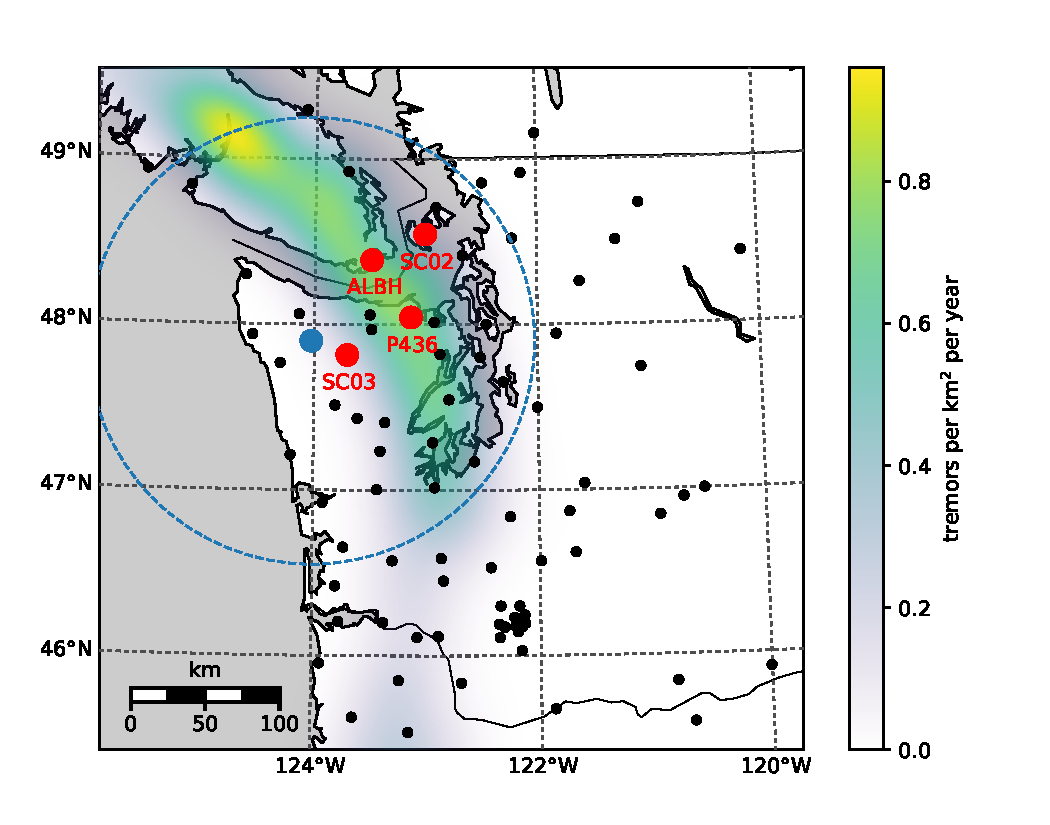
\includegraphics{figures/context_map/context-map.pdf}
\caption{
Positions of \DIFdelbeginFL \DIFdelFL{continuous }\DIFdelendFL \DIFaddbeginFL \DIFaddFL{the }\DIFaddendFL GNSS stations used to estimate transient strain
rates. The colored regions indicate the distribution of seismic tremor
as determined by \citet{Wech2010}. The red dots show the positions of
GNSS stations mentioned in this paper. The blue dot indicates the
location of the transient strain rates shown in Figure
\ref{fig:StrainTs} and the signal-to-noise ratio shown in Figure
\ref{fig:StrainMag}. The blue dashed circle demarcates the spatial
extent of the tremors shown in Figure \ref{fig:StrainMag}.
}    
\label{fig:Context}
\end{figure*}

%DIF > % NOISE MODEL
\subsection{Noise model}\label{sec:NoiseModel}
\DIFdelbegin \DIFdel{Before we determine the transient strain rates, we must establish a
prior for the transient displacements, $u$, and the noise, $\eta$. In this section we discuss our choice for the noise covariance function $C_\eta$. There have been numerous studies on }\DIFdelend \DIFaddbegin 

%DIF >  Defining the components of the noise vector

\DIFadd{We consider the noise vector, $\mitbf{\eta}_i$, to be composed of a
temporally correlated Gaussian process, $z_i \sim
\mathcal{GP}(0,C_{z_i})$, and a vector of uncorrelated
Gaussian noise, $\mitbf{w}_i$, so that
}\begin{equation}
\DIFadd{\mitbf{\eta}_i = z_i(\points) + \mitbf{w}_i.
}\end{equation}
\DIFadd{The standard deviations for $\mitbf{w}_i$ are taken to be the
uncertainties derived for the GNSS displacement solutions,
$\mitbf{\sigma}_i$. The noise vector then has zero mean and the
covariance matrix
}\begin{equation}
\DIFadd{\mitbf{C}_{\eta_i} = C_{z_i}(\points,\points) +
                     \mathrm{diag}(\mitbf{\sigma}_i^2).
}\end{equation}

%DIF >  Justifying our temporal noise model

\DIFadd{The }\DIFaddend temporally correlated noise in GNSS data \DIFdelbegin \DIFdel{\mbox{%DIFAUXCMD
\citep[e.g.,][]{Zhang1997,Mao1999,Williams2004,Langbein2008}}%DIFAUXCMD
}\DIFdelend \DIFaddbegin \DIFadd{has been thoroughly
studied over the past two decades \mbox{%DIFAUXCMD
\citep[e.g.,][]{Zhang1997, Mao1999,
Williams2004, Langbein2008}}%DIFAUXCMD
}\DIFaddend . In these studies, temporally correlated
noise \DIFdelbegin \DIFdel{was }\DIFdelend \DIFaddbegin \DIFadd{tends to be }\DIFaddend described with some combination of Brownian motion
\DIFaddbegin \DIFadd{(also known as random walk noise or a Weiner process)}\DIFaddend , a first-order
Gauss-Markov (FOGM) process, and/or flicker noise. There is some
physical justification for using Brownian motion as a noise model
because it accurately describes the power spectrum of motion resulting
from instability in \DIFdelbegin \DIFdel{geodetic monuments \mbox{%DIFAUXCMD
\citep[e.g.,][]{Wyatt1982,Wyatt1989}}%DIFAUXCMD
. Here we describe the time dependence of $\eta$ as a FOGM process and
consider $\eta$ to be spatially uncorrelated. A FOGM process is
a solution to the stochastic differential equation
}\begin{displaymath}\DIFdel{%DIFDELCMD < \label{eq:FOGMdef}%%%
\dot{\eta}(t) + \alpha \eta(t) = \beta w(t),
}\end{displaymath}
%DIFAUXCMD
\DIFdel{where $w(t)$ is white noise with unit variance. The FOGM process degenerates to the commonly used Brownian motion noise model under the condition that $\alpha=0$ and $\eta(0) = 0$.Our noise model that satisfies eq.(\ref{eq:FOGMdef}) is a Gaussian processwith zero mean and }\DIFdelend \DIFaddbegin \DIFadd{a geodetic monument \mbox{%DIFAUXCMD
\citep[e.g.,][]{Wyatt1982,
Wyatt1989}}%DIFAUXCMD
. In particular, the power spectrums for Brownian motion and
monument motion both decay proportionally to $f^{-2}$, where $f$ is
frequency. However, Brownian motion necessarily contains a reference
time at which the process begins. Since there is no notion of when
noise ``begins" in GNSS data, we do not find Brownian motion to be an
appropriate noise model. On the other hand, a FOGM process has no
reference time (i.e., it is stationary), and its power spectrum,
}\begin{equation}\DIFadd{\label{eq:FOGMPS}
S(f) = \frac{\beta^2}{(2 \pi f)^2 + \alpha^2},
}\end{equation}
\DIFadd{decays proportionally to $f^{-2}$ above the cutoff frequency $\alpha /
(2 \pi)$. We then choose $z_i$ to be a spatially
uncorrelated FOGM process, which has }\DIFaddend the covariance function
\begin{equation}\label{eq:FOGM}
C\DIFdelbegin \DIFdel{_\eta}\DIFdelend \DIFaddbegin \DIFadd{_{z_i}}\DIFaddend \left((\DIFdelbegin %DIFDELCMD < \vec{x}%%%
\DIFdelend \DIFaddbegin \pos\DIFaddend ,t),(\DIFdelbegin %DIFDELCMD < \vec{x}%%%
\DIFdelend \DIFaddbegin \pos\DIFaddend ',t')\right) = 
\frac{\beta^2}{2\alpha}
\exp\left(-\alpha|t - t'|\right)\delta\DIFdelbegin \DIFdel{(||}%DIFDELCMD < \vec{x} %%%
\DIFdel{- }%DIFDELCMD < \vec{x}%%%
\DIFdel{'||_2). 
}\DIFdelend \DIFaddbegin \DIFadd{_{\pos,\pos'},
}\DIFaddend \end{equation}
\DIFaddbegin \DIFadd{where $\delta_{\pos,\pos'}$ is 1 if $\pos = \pos'$ and 0 otherwise.
See \mbox{%DIFAUXCMD
\citet[sec. B2]{Rasmussen2006} }%DIFAUXCMD
for more information on the FOGM
process.
}\DIFaddend 

\DIFdelbegin \DIFdel{We constrain the hyperparameters for $\eta$}\DIFdelend %DIF >  How we constrain the parameters
\DIFaddbegin 

\DIFadd{By choosing a FOGM process for $z_i$, we have introduced two
parameters that need to be constrained}\DIFaddend , $\alpha$ and $\beta$\DIFdelbegin \DIFdel{, with a set of }\DIFdelend \DIFaddbegin \DIFadd{. We
constrain these parameters, which we collectively refer to as
$\mitbf{\theta}$, with the Restricted Maximum Likelihood (REML) method
\mbox{%DIFAUXCMD
\citep{Harville1974}}%DIFAUXCMD
. The REML method is conceptually similar to the
Maximum Likelihood Estimation (MLE) method from \mbox{%DIFAUXCMD
\citet{Langbein1997}}%DIFAUXCMD
,
where we pick $\mitbf{\theta}$ to maximize the probability of drawing
the observed data, $\mitbf{d}_i^*$, from the random vector
$\mitbf{d}_i$. However, unlike the MLE method, the REML method
produces unbiased estimates of $\mitbf{\theta}$ \mbox{%DIFAUXCMD
\citep[sec.
2.6]{Cressie1992}}%DIFAUXCMD
. We use the REML method to estimate $\mitbf{\theta}$
at }\DIFaddend 38 continuous GNSS stations in \DIFdelbegin \DIFdel{Cascadia }\DIFdelend \DIFaddbegin \DIFadd{the Pacific Northwest }\DIFaddend that are east
of 121$^\circ$W. These stations are sufficiently far from the
subduction zone that they are unlikely to \DIFdelbegin \DIFdel{contain transient signal associated with SSEs.  We clean the data for these stations by removing jumps at times of equipment changes, and we remove outliers that have been detected with the algorithm described in Section \ref{sec:Outlier}. We then find $\alpha$ and $\beta$ for each
station time series with the Restricted Maximum Likelihood (REML ) method \mbox{%DIFAUXCMD
\cite[e.g.,][]{Harville1974,Cressie1992,Hines2017}}%DIFAUXCMD
. The REML method finds the hyperparameters, which we collectively refer to as }\DIFdelend \DIFaddbegin \DIFadd{record transient deformation
from SSEs, allowing us to ingore the term $u_i(\points)$ in
$\mitbf{d}_i$. We assume the noise at these inland stations is
representative of the noise at all the stations considered in this
study, which is probably a poor assumption since the inland stations
are subject to distinctly different climatic conditions. Nonetheless,
we find $\mitbf{\theta}$ for each of the inland stations and for each
displacement component by maximizing the REML likelihood function
}\begin{equation}\DIFadd{\label{eq:REMLNoise}
\mathcal{L}(\mitbf{\theta}) = \left(\frac{\left|\G^T\G\right|}{(2\pi)^{n-6m} 
                                    \left| \mitbf{C}_{\eta_i}(\mitbf{\theta}) \right| 
                                    \left| \G^T\mitbf{C}_{\eta_i}(\mitbf{\theta})^{-1}\G \right|}\right)^{\frac{1}{2}} 
                              e^{-\tfrac{1}{2}\data_i^{*T}\mitbf{K}(\mitbf{\theta})\data_i^*}
}\end{equation}
\DIFadd{with respect to }\DIFaddend $\mitbf{\theta}$, \DIFdelbegin \DIFdel{that maximize the likelihood function
}\begin{displaymath}\DIFdel{%DIFDELCMD < \label{eq:REML}%%%
\mathcal{L}(\mitbf{\theta}) = \left(\frac{\left|\mitbf{G}^T\mitbf{G}\right|}{(2\pi)^{n-6m} 
                           \left| \mitbf{\Sigma}(\mitbf{\theta}) \right| 
                           \left| \mitbf{G}^T\mitbf{\Sigma}(\mitbf{\theta})^{-1}\mitbf{G} \right|}\right)^{\frac{1}{2}} 
                           e^{-\tfrac{1}{2}\mitbf{d}_*^T\mitbf{K}(\mitbf{\theta})\mitbf{d}_*},
}\end{displaymath}
%DIFAUXCMD
\DIFdel{where
}\DIFdelend \DIFaddbegin \DIFadd{where
}\DIFaddend \begin{equation}
\mitbf{K}(\mitbf{\theta}) = \DIFdelbegin %DIFDELCMD < \mitbf{\Sigma}%%%
\DIFdelend \DIFaddbegin \mitbf{C}\DIFadd{_{\eta_i}}\DIFaddend (\mitbf{\theta})^{-1} - 
                            \DIFdelbegin %DIFDELCMD < \mitbf{\Sigma}%%%
\DIFdelend \DIFaddbegin \mitbf{C}\DIFadd{_{\eta_i}}\DIFaddend (\mitbf{\theta})^{-1}\DIFdelbegin %DIFDELCMD < \mitbf{G}
%DIFDELCMD <          %%%
\DIFdelend \DIFaddbegin \G
                            \DIFaddend \left(\DIFdelbegin %DIFDELCMD < \mitbf{G}%%%
\DIFdelend \DIFaddbegin \G\DIFaddend ^T\DIFdelbegin %DIFDELCMD < \mitbf{\Sigma}%%%
\DIFdelend \DIFaddbegin \mitbf{C}\DIFadd{_{\eta_i}}\DIFaddend (\mitbf{\theta})^{-1}\DIFdelbegin %DIFDELCMD < \mitbf{G}%%%
\DIFdelend \DIFaddbegin \G\DIFaddend \right)^{-1}
                            \DIFdelbegin %DIFDELCMD < \mitbf{G}%%%
\DIFdelend \DIFaddbegin \G\DIFaddend ^T\DIFdelbegin %DIFDELCMD < \mitbf{\Sigma}%%%
\DIFdelend \DIFaddbegin \mitbf{C}\DIFadd{_{\eta_i}}\DIFaddend (\mitbf{\theta})^{-1}.
\end{equation}
\DIFdelbegin \DIFdel{\mbox{%DIFAUXCMD
\citet{Harville1974} }%DIFAUXCMD
showed that choosing the hyperparameters which maximize eq. (\ref{eq:REML}) is equivalent to choosing the hyperparameters which maximize the probability of drawing $\mitbf{d}_*$ from $\mitbf{d}$. We independently estimate $\mitbf{\theta}$ for each station, and so $\mitbf{d}_*$ consists of displacements for an individual station. We are assuming $u(p)=0$ when estimating the noise hyperparameters for this section. We use the REML method over the maximum likelihood (ML) method \mbox{%DIFAUXCMD
\citep[e.g.,][]{Langbein1997} }%DIFAUXCMD
because the REML method accounts for the improper prior that we assigned to $\mitbf{a}$ \mbox{%DIFAUXCMD
\citep{Hines2017}}%DIFAUXCMD
.
}\DIFdelend \DIFaddbegin \DIFadd{In the above equation, $\data^*_i$ consists of the data for a single station.
}

%DIF >  results of estimated parameters

\DIFaddend The distribution of inferred \DIFaddbegin \DIFadd{values for }\DIFaddend $\alpha$ and $\beta$ are shown
in Figure \ref{fig:NoiseParams}. The \DIFdelbegin \DIFdel{amplitude of FOGM noise, }\DIFdelend \DIFaddbegin \DIFadd{estimates of }\DIFaddend $\beta$ \DIFdelbegin \DIFdel{, }\DIFdelend for the
easting and northing components \DIFdelbegin \DIFdel{is notable low and }\DIFdelend are clustered around 0.5
mm/yr$^{0.5}$. The corresponding estimates of $\alpha$ tend to cluster
around 0 yr$^{-1}$, \DIFdelbegin \DIFdel{suggesting that noise can be described with Brownian motion}\DIFdelend \DIFaddbegin \DIFadd{indicating that the power spectrum of noise indeed
decays proportionally to $f^{-2}$ over a wide band of frequencies}\DIFaddend . We
also estimate \DIFdelbegin \DIFdel{hyperparameters }\DIFdelend \DIFaddbegin \DIFadd{$\alpha$ and $\beta$ }\DIFaddend for the vertical component of
displacements, \DIFdelbegin \DIFdel{under }\DIFdelend \DIFaddbegin \DIFadd{with }\DIFaddend the hope that vertical deformation gradients could
reveal some geophysical signal. \DIFdelbegin \DIFdel{The amplitude of FOGM noise for }\DIFdelend \DIFaddbegin \DIFadd{For }\DIFaddend the vertical component\DIFaddbegin \DIFadd{, $\beta$ }\DIFaddend is
relatively large with a median value of 13.5 mm/yr$^{0.5}$. The
inferred values for $\alpha$ are also higher for the vertical
component with a median value of 8.21 yr$^{-1}$. In Figure
\ref{fig:NoiseSamples}, we use the median values of $\alpha$ and
$\beta$ to generate two \DIFdelbegin \DIFdel{random samples }\DIFdelend \DIFaddbegin \DIFadd{realizations }\DIFaddend of FOGM noise for each component.
The \DIFdelbegin \DIFdel{samples }\DIFdelend \DIFaddbegin \DIFadd{realizations }\DIFaddend span five years\DIFdelbegin \DIFdel{and over these five years }\DIFdelend \DIFaddbegin \DIFadd{, and }\DIFaddend the easting and northing
\DIFdelbegin \DIFdel{samples }\DIFdelend \DIFaddbegin \DIFadd{realizations }\DIFaddend drift by about 1 mm \DIFaddbegin \DIFadd{over these five years}\DIFaddend . In the context
of detecting SSEs, which produce several mm's of surface displacement
on the time-scale of weeks, the estimated FOGM noise for the easting
and northing component is negligible. In contrast, the estimated FOGM
noise for the vertical component is larger than the signal we would
expect from SSEs. We suspect that the higher amplitude for the FOGM
noise in the vertical component is accommodating for deficiencies in
our rather simple seasonal model. Based on this analysis, we
henceforth ignore temporally correlated noise in the easting and
northing component because of its low amplitude. We also do not use
vertical displacements because of the presumably low signal-to-noise
ratio.

\begin{figure*}
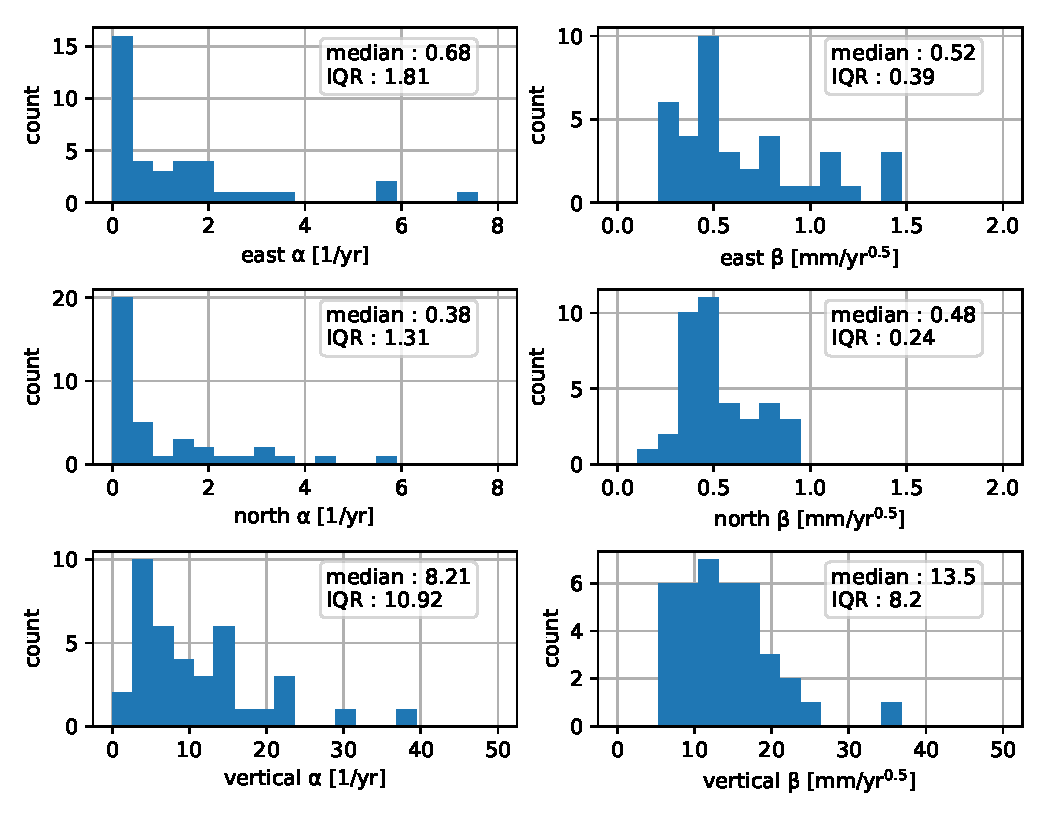
\includegraphics{figures/noise/noise-params.pdf}
\caption{
Distribution of \DIFdelbeginFL \DIFdelFL{estimated }\DIFdelendFL \DIFaddbeginFL \DIFaddFL{inferred values for the parameters in the }\DIFaddendFL FOGM \DIFdelbeginFL \DIFdelFL{hyperparameters }\DIFdelendFL \DIFaddbeginFL \DIFaddFL{noise
model }\DIFaddendFL (eq. \ref{eq:FOGM}). \DIFdelbeginFL \DIFdelFL{Hyperparameters are estimated with the REML method for 38 stations in Cascadia that are east of $121^\circ$W. }\DIFdelendFL ``IQR'' is the interquartile range \DIFaddbeginFL \DIFaddFL{of
inferred values}\DIFaddendFL .
}   
\label{fig:NoiseParams}
\end{figure*}

\begin{figure*}
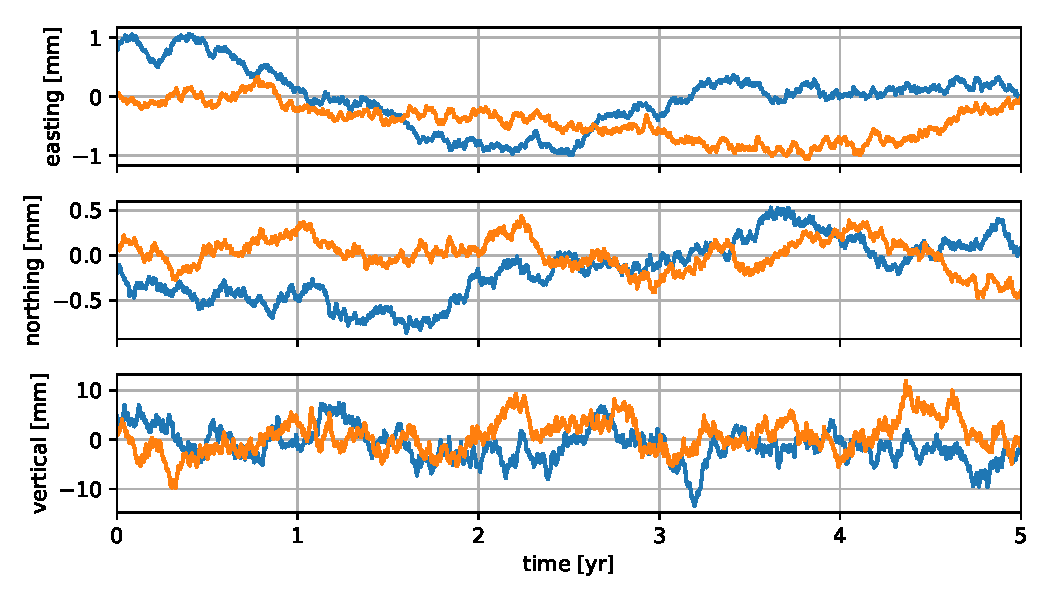
\includegraphics{figures/noise/noise-samples.pdf}
\caption{
Two \DIFaddbeginFL \DIFaddFL{samples of }\DIFaddendFL FOGM noise \DIFdelbeginFL \DIFdelFL{samples }\DIFdelendFL for each \DIFaddbeginFL \DIFaddFL{displacement }\DIFaddendFL component. The
\DIFaddbeginFL \DIFaddFL{parameters for the }\DIFaddendFL FOGM \DIFdelbeginFL \DIFdelFL{hyperparameters }\DIFdelendFL \DIFaddbeginFL \DIFaddFL{noise model }\DIFaddendFL have been set to the median values
from Figure \ref{fig:NoiseParams}.
}   
\label{fig:NoiseSamples}
\end{figure*}

%DIF >  Note spatially correlated noise
\DIFaddbegin 

\DIFaddend Another significant source of noise in GNSS data is common mode error
\citep[e.g.,][]{Wdowinski1997,Dong2006}, which is noise that is highly
spatially correlated. When not accounted for, common mode error
manifests as spatially uniform undulations in \DIFaddbegin \DIFadd{our }\DIFaddend estimated transient
displacements. \DIFdelbegin \DIFdel{However, estimated }\DIFdelend \DIFaddbegin \DIFadd{These undulations have no effect on the }\DIFaddend transient
strain rates\DIFdelbegin \DIFdel{are insensitive to common mode error. We therefore do not }\DIFdelend \DIFaddbegin \DIFadd{, and so we do not need to }\DIFaddend include common mode error in
our noise model.
\DIFdelbegin \DIFdel{We then make the simplifying assumption that $\eta(p) = 0$ for the easting and northing component of GNSS data.  
}\DIFdelend 

%DIF > % PRIOR MODEL
\subsection{Prior model}\label{sec:SignalModel}
\DIFaddbegin 

%DIF >  State our choice for X_i

\DIFaddend We next establish \DIFdelbegin \DIFdel{our }\DIFdelend \DIFaddbegin \DIFadd{a }\DIFaddend prior model for transient displacements.
Specifically, we discuss our choice for the \DIFdelbegin \DIFdel{covariance functions $X(\vec{x},\vec{x}')$ and $T(t,t')$. For $X$}\DIFdelend \DIFaddbegin \DIFadd{spatial and temporal
functions making up $C_{u_i}$, $X_i$ and $T_i$. For $X_i$}\DIFaddend , we use the
squared exponential (SE) covariance function,
\begin{equation}\label{eq:SE}
X\DIFaddbegin \DIFadd{_i}\DIFaddend (\DIFdelbegin %DIFDELCMD < \vec{x}%%%
\DIFdelend \DIFaddbegin \pos\DIFaddend ,\DIFdelbegin %DIFDELCMD < \vec{x}%%%
\DIFdelend \DIFaddbegin \pos\DIFaddend ') = \exp\left(\DIFdelbegin \DIFdel{\frac{-||\vec{x} - \vec{x}'||_2^2}{2 \ell^2}}\DIFdelend \DIFaddbegin \DIFadd{\frac{-||\pos - \pos'||_2^2}{2 \ell^2}}\DIFaddend \right).
\end{equation}
The SE covariance function is commonly used \DIFdelbegin \DIFdel{in }\DIFdelend \DIFaddbegin \DIFadd{for }\DIFaddend kriging
\citep[e.g,][]{Cressie1992} and Gaussian process regression
\citep[e.g.,][]{Rasmussen2006}. \DIFdelbegin \DIFdel{The SE is a positive definite covariance function for any number of spatial dimensions. A Gaussian process with an SE covariance function is isotropic and has realizations that are infinitely differentiable. }\DIFdelend In terms of geodetic applications,
\citet{Kato1998} and \cite{El-Fiky1999} demonstrated that the SE
\DIFaddbegin \DIFadd{covariance function }\DIFaddend accurately describes the \DIFaddbegin \DIFadd{spatial }\DIFaddend covariance of
secular GNSS derived velocities in Japan.

%DIF >  List our choices for T_i
\DIFaddbegin 

\DIFaddend We consider three potential \DIFdelbegin \DIFdel{models for the temporal covariance of $u$. First, we consider }\DIFdelend \DIFaddbegin \DIFadd{choices for $T_i$. The first option is }\DIFaddend the
one-dimensional SE covariance function,
\begin{equation}\label{eq:TimeSE}
T\DIFaddbegin \DIFadd{_i}\DIFaddend (t,t') = \phi^2\exp\left(\frac{-|t - t'|^2}{2\tau^2}\right).
\end{equation}
Note that \DIFdelbegin \DIFdel{$T$ includes the hyperparameter }\DIFdelend \DIFaddbegin \DIFadd{$T_i$ includes the parameter }\DIFaddend $\phi$, which serves to scale
the covariance function \DIFdelbegin \DIFdel{$C_u$. Second, we
consider }\DIFdelend \DIFaddbegin \DIFadd{$C_{u_i}$. The second option is a member of
the Wendland class of covariance functions \mbox{%DIFAUXCMD
\citep{Wendland2005}}%DIFAUXCMD
.
Wendland covariance functions have compact support and hence their
corresponding covariance matrices are sparse. In our analysis, we
exploit this sparsity with the CHOLMOD software package
\mbox{%DIFAUXCMD
\citep{Chen2008}}%DIFAUXCMD
. Wendland covariance functions can be constructed
such that they are positive definite in $\mathbb{R}^d$ and their
corresponding Gaussian process can be differentiated $k$ times. We use
$d=1$, because we are describing the temporal covariance of $u_i$, and
we use $k=2$, giving samples of $u_i$ continuous velocities and
accelerations. The corresponding Wendland covariance function is
}\begin{equation}\DIFadd{\label{eq:Wendland} 
T_i(t,t') = \phi^2\left(1 - \frac{|t - t'|}{\tau}\right)^5_+ 
            \left(\frac{8|t - t'|^2}{\tau^2} + \frac{5|t - t'|}{\tau} + 1\right), 
}\end{equation} 
\DIFadd{where $(t)_+ = \mathrm{max}(0,t)$. The third option for $T_i$ is the
covariance function for }\DIFaddend integrated Brownian motion (IBM). IBM \DIFdelbegin \DIFdel{has }\DIFdelend \DIFaddbegin \DIFadd{is a
Gaussian process with }\DIFaddend zero mean and its covariance function can be
found by integrating the covariance function for Brownian motion\DIFdelbegin \DIFdel{as
}\DIFdelend \DIFaddbegin \DIFadd{,
}\DIFaddend \begin{align}\label{eq:IBM}
T\DIFaddbegin \DIFadd{_i}\DIFaddend (t,t') &= \int_0^t \int_0^{t'} \phi^2 \min(s,s') \,ds'\,ds \\
          &= \frac{\phi^2}{2}\min(t,t')^2 \left(\max(t,t') - \frac{1}{3}\min(t,t')\right), \ \ \ t,t' \geq 0.
\end{align}
IBM has been used in the context of Kalman filtering as a
non-parametric model for the time dependence of geophysical signals
\DIFdelbegin \DIFdel{\mbox{%DIFAUXCMD
\citep[e.g.,][]{Segall1997,McGuire2003,Ohtani2010,Hines2016a}}%DIFAUXCMD
.
It should be emphasized $t=0$ is }\DIFdelend \DIFaddbegin \DIFadd{\mbox{%DIFAUXCMD
\citep[e.g.,][]{Segall1997, McGuire2003, Ohtani2010, Hines2016a}}%DIFAUXCMD
.
Similar to Brownian motion, IBM has }\DIFaddend a reference time\DIFaddbegin \DIFadd{, $t=0$, }\DIFaddend at which
the \DIFdelbegin \DIFdel{Gaussian process is exactly zero}\DIFdelend \DIFaddbegin \DIFadd{process begins}\DIFaddend . For some geophysical signals, it is appropriate to
have this reference time. For example, if we are trying to identify
postseismic deformation then $t$ should be zero at the time of the
earthquake.  However, if we are \DIFdelbegin \DIFdel{interesting }\DIFdelend \DIFaddbegin \DIFadd{interested }\DIFaddend in detecting transient
events, where there is no known start time, then IBM may not be an
appropriate prior \DIFdelbegin \DIFdel{, and an isotropic Gaussian process should be preferred}\DIFdelend \DIFaddbegin \DIFadd{model. Instead, one may prefer to use the SE or
Wendland covariance functions because they are stationary}\DIFaddend . In the
following analysis, we make the \DIFdelbegin \DIFdel{quite arbitrary }\DIFdelend choice that $t$ is zero on the first
epoch of \DIFdelbegin \DIFdel{$\mitbf{d}_*$}\DIFdelend \DIFaddbegin \DIFadd{$\data_i^*$}\DIFaddend . Using an earlier reference time does not change
the results discussed in this section.
\DIFdelbegin \DIFdel{Our third option for $T$ is the Wendland class of covariance functions \mbox{%DIFAUXCMD
\citep{Wendland2005}}%DIFAUXCMD
. Wendland covariance functions have compact support and hence their corresponding covariance matrices will be sparse. In our analysis, we exploit this sparsity with the CHOLMOD software package \mbox{%DIFAUXCMD
\citep{Chen2008}}%DIFAUXCMD
. Wendland functions are positive definite in $\mathbb{R}^d$, and they describes an isotropic Gaussian process with realizations that can be differentiated $k$ times. The form of the covariance function depends on the choice of $d$ and $k$. We use $d=1$ since we are describing the temporal covariance of $u$. We use $k=2$, giving samples of $u$ continuous velocities and accelerations. The corresponding Wendland covariance function is 
}\begin{displaymath}\DIFdel{%DIFDELCMD < \label{eq:Wendland}%%%
T(t,t') = \phi^2\left(1 - \frac{|t - t'|}{\tau}\right)^5_+ \left(\frac{8|t - t'|^2}{\tau^2} + \frac{5|t - t'|}{\tau} + 1\right), 
}\end{displaymath}
%DIFAUXCMD
\DIFdel{where
}\begin{displaymath}
\DIFdel{(t)_+ = 
\begin{cases}
t, \ \ \ t > 0 \\
0, \ \ \ \mathrm{otherwise}.
\end{cases}
}\end{displaymath}
%DIFAUXCMD
\DIFdelend 

\DIFdelbegin \DIFdel{We next determine appropriate hyperparameters for $X$ and each of the three candidate covariance functions for $T$. First, we clean the
GNSS datasets by removing offsets at times of equipment changes and removing outliers with the method describe in Section \ref{sec:Outlier}. For the outlier detection algorithm, our prior model, $u$, is chosen to have a length-scale and time-scale which is able to approximately describe SSE displacements. We
use the SE covariance function for $X$ with length-scale $\ell = 100$ km, and we use the Wendland covariance function for $T$, due to its computational efficiency, with time-scale $\tau = 0.1$ yr and $\phi = 1$ mm. The outlier detection algorithm is particularly effective at removing outliers for stations at high elevation (Figure \ref{fig:Outliers}), which can be adversely affected by ice or snow during the
winter \mbox{%DIFAUXCMD
\citep{Lisowski2008}}%DIFAUXCMD
. After cleaning the dataset, we divide
it }\DIFdelend %DIF >  Choosing the parameters
\DIFaddbegin 

\DIFadd{We use the REML method to determine the appropriate values for the
parameters in $C_{u_i}$, which are $\ell$, $\phi$, and $\tau$. We
refer to these parameters collectively as $\mitbf{\theta}$. Just as in
Section \ref{sec:NoiseModel}, we pick $\mitbf{\theta}$ to maximize the
probability of drawing $\data_i^*$ from $\data_i$, but now we are
including $u_i(\points)$ in $\data_i$. and we are optimizing the
parameters for $C_{u_i}$ rather than $\mitbf{C}_{\eta_i}$. We divide
the GNSS data }\DIFaddend into seven subsets \DIFdelbegin \DIFdel{which }\DIFdelend \DIFaddbegin \DIFadd{that }\DIFaddend are four months long and each
centered on the time of a SSE. The times of the seven SSEs are
determined with tremor records from \cite{Wech2010}. We \DIFdelbegin \DIFdel{use the REML method to }\DIFdelend find the
optimal \DIFdelbegin \DIFdel{hyperparameters for $T$ and $X$ }\DIFdelend \DIFaddbegin \DIFadd{$\mitbf{\theta}$ }\DIFaddend for each subset of data\DIFdelbegin \DIFdel{. We choose to make each
data subsets four months long because it is long enough to encompass a SSE in Cascadia, while it is short enough to still be computationally tractable. However, four months is too short to
resolve the sinusoids in $\mitbf{d}$,
and they are omitted from $\mitbf{d}$ in this REML analysis for Cascadia SSEs}\DIFdelend \DIFaddbegin \DIFadd{, for each
displacement component, and for each choice of $T_i$. The REML
likelihood function that we are maximizing with respect to
$\mitbf{\theta}$ is now
}\begin{equation}\DIFadd{\label{eq:REMLPrior} 
\mathcal{L}(\mitbf{\theta}) =
\left(\frac{\left| \G^T \G \right|}{(2\pi)^{n-6m}
                                    \left| \mitbf{\Sigma}(\mitbf{\theta}) \right| 
                                    \left| \G^T \mitbf{\Sigma}(\mitbf{\theta})^{-1} \G \right|}\right)^{\frac{1}{2}} 
                              e^{-\tfrac{1}{2} \data_i^{*T} \mitbf{K}(\mitbf{\theta}) \data_i^*},
}\end{equation}
\DIFadd{where
}\begin{equation}
\DIFadd{\mitbf{K}(\mitbf{\theta}) = \mitbf{\Sigma}(\mitbf{\theta})^{-1} - 
                            \mitbf{\Sigma}(\mitbf{\theta})^{-1} \G
                            \left( \G^T \mitbf{\Sigma}(\mitbf{\theta})^{-1} \G \right)^{-1}
                            \G^T \mitbf{\Sigma}(\mitbf{\theta})^{-1}
}\end{equation}
\DIFadd{and $\mitbf{\Sigma}(\mitbf{\theta}) = \mitbf{C}_{\eta_i} +
C_{u_i}(\points,\points;\mitbf{\theta})$. In the above equation,
$\data^*_i$ consists of a single subset of data}\DIFaddend . The estimated
\DIFdelbegin \DIFdel{hyperparameters for $u$ }\DIFdelend \DIFaddbegin \DIFadd{parameters }\DIFaddend are summarized in Table 1. Based on the interquartile
ranges, the estimated \DIFdelbegin \DIFdel{hyperparameters }\DIFdelend \DIFaddbegin \DIFadd{parameters }\DIFaddend for the SE and Wendland covariance
functions do not vary significantly between SSEs. This suggests that
the median of \DIFdelbegin \DIFdel{estimated hyperparameters should be an appropriate prior model for all
Cascadia }\DIFdelend \DIFaddbegin \DIFadd{the estimated parameters should be appropriate for all
the Pacific Northwest }\DIFaddend SSEs. For the IBM model, there are several
anomalously large values for $\ell$ and $\phi$, which \DIFdelbegin \DIFdel{results in large interquartile ranges }\DIFdelend \DIFaddbegin \DIFadd{is why the
interquartile ranges are large}\DIFaddend .

\DIFdelbegin %DIFDELCMD < \begin{figure*}
%DIFDELCMD < 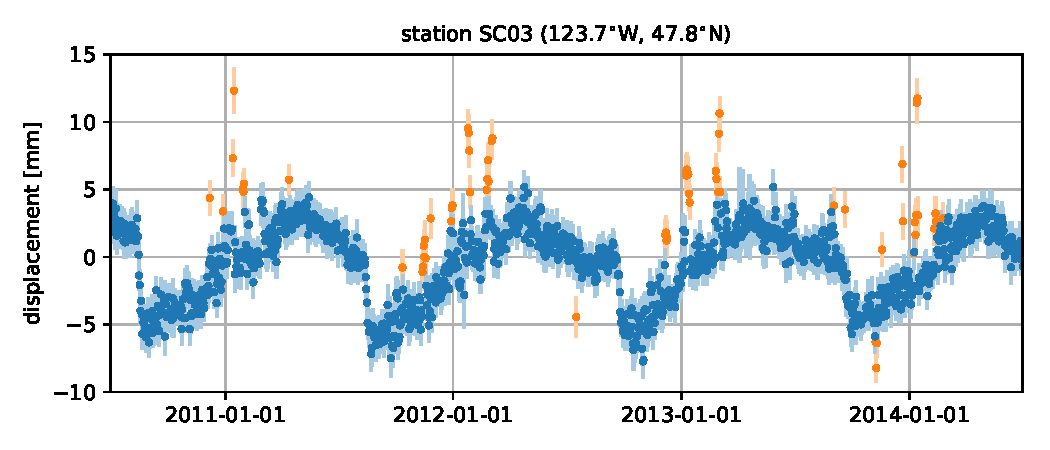
\includegraphics{figures/outliers/outliers.pdf}
%DIFDELCMD < %%%
%DIFDELCMD < \caption{%
{%DIFAUXCMD
\DIFdelFL{Detrended easting component of displacements at station SC03, which is located on Mount Olympus in Washington. The orange markers indicate outliers that were automatically detected using the algorithm from Section \ref{sec:Outlier}. The error bars show one standard deviation uncertainties. Note that outliers tend be observed in the winter, suggesting that they were caused by snow or ice.}}   
%DIFAUXCMD
%DIFDELCMD < %DIFDELCMD < \label{fig:Outliers}%%%
%DIFDELCMD < \end{figure*}
%DIFDELCMD < 

%DIFDELCMD < %%%
\DIFdelend \begin{table}\label{tab:Parameters}
\caption{
Optimal \DIFdelbeginFL \DIFdelFL{hyperparameters }\DIFdelendFL \DIFaddbeginFL \DIFaddFL{values }\DIFaddendFL for the \DIFdelbeginFL \DIFdelFL{prior on transient displacements }\DIFdelendFL \DIFaddbeginFL \DIFaddFL{parameters in $X_i$ and $T_i$ }\DIFaddendFL determined with
the REML method. The \DIFdelbeginFL \DIFdelFL{temporal }\DIFdelendFL covariance function \DIFaddbeginFL \DIFaddFL{for $T_i$ }\DIFaddendFL is indicated by the
``\DIFdelbeginFL \DIFdelFL{$T$}\DIFdelendFL \DIFaddbeginFL \DIFaddFL{$T_i$}\DIFaddendFL '' column. The SE, \DIFdelbeginFL \DIFdelFL{IBM}\DIFdelendFL \DIFaddbeginFL \DIFaddFL{Wendland}\DIFaddendFL , and \DIFdelbeginFL \DIFdelFL{Wendland }\DIFdelendFL \DIFaddbeginFL \DIFaddFL{IBM }\DIFaddendFL covariance functions are
defined in eqs. (\ref{eq:TimeSE}), (\DIFdelbeginFL \DIFdelFL{\ref{eq:IBM}}\DIFdelendFL \DIFaddbeginFL \DIFaddFL{\ref{eq:Wendland}}\DIFaddendFL ), and
(\DIFdelbeginFL \DIFdelFL{\ref{eq:Wendland}}\DIFdelendFL \DIFaddbeginFL \DIFaddFL{\ref{eq:IBM}}\DIFaddendFL ), respectively. \DIFdelbeginFL \DIFdelFL{The spatial covariance function, $X$, is the squared exponential (}\DIFdelendFL \DIFaddbeginFL \DIFaddFL{We use }\DIFaddendFL eq. \DIFaddbeginFL \DIFaddFL{(}\DIFaddendFL \ref{eq:SE}) \DIFdelbeginFL \DIFdelFL{in all cases}\DIFdelendFL \DIFaddbeginFL \DIFaddFL{for $X_i$}\DIFaddendFL .
The \DIFdelbeginFL \DIFdelFL{hyperparameters }\DIFdelendFL \DIFaddbeginFL \DIFaddFL{parameters }\DIFaddendFL are estimated for each of the seven SSEs considered in
this study, and the tabulated values indicate the median and
interquartile ranges of \DIFdelbeginFL \DIFdelFL{estimates}\DIFdelendFL \DIFaddbeginFL \DIFaddFL{estimated values}\DIFaddendFL . The ``diff $\log$(REML)'' column
compares the \DIFaddbeginFL \DIFaddFL{optimal }\DIFaddendFL log REML \DIFdelbeginFL \DIFdelFL{likelihood }\DIFdelendFL \DIFaddbeginFL \DIFaddFL{likelihoods }\DIFaddendFL to \DIFdelbeginFL \DIFdelFL{the log REML likelihood }\DIFdelendFL \DIFaddbeginFL \DIFaddFL{those for }\DIFaddendFL when \DIFdelbeginFL \DIFdelFL{using }\DIFdelendFL \DIFaddbeginFL \DIFaddFL{$T_i$ is
}\DIFaddendFL the SE covariance function\DIFdelbeginFL \DIFdelFL{for $T$}\DIFdelendFL . Negative values indicate that observations
are more consistent with the SE covariance function.
} 
\begin{tabular} {l l l l l l}
\DIFdelbeginFL \DIFdelFL{$T$ }\DIFdelendFL \DIFaddbeginFL \DIFaddFL{$T_i$ }\DIFaddendFL & \DIFdelbeginFL \DIFdelFL{direction }\DIFdelendFL \DIFaddbeginFL \DIFaddFL{component }\DIFaddendFL & $\ell$  & $\phi$   & $\tau$  & diff. $\log$(REML) \\ \hline
SE & east   & 92 $\pm$ 25 km  & 0.62 $\pm$ 0.11 mm  & 0.026 $\pm$ 0.011 yr  &  - \\
SE & north  & 91 $\pm$ 53 km  & 0.43 $\pm$ 0.05 mm  & 0.030 $\pm$ 0.017 yr  &  - \\
Wendland & east   & 95 $\pm$ 30 km  & 0.66 $\pm$ 0.15 mm  & 0.093 $\pm$ 0.044 yr &  0.78 $\pm$ 0.87 \\
Wendland & north  & 92 $\pm$ 57 km  & 0.46 $\pm$ 0.10 mm  & 0.116 $\pm$ 0.057 yr &  0.08 $\pm$ 0.58 \\
IBM & east   & 110 $\pm$ 130 km & 290 $\pm$ 420 mm/yr$^{1.5}$  & -          & -16.4 $\pm$ 7.8 \\
IBM & north  & 150 $\pm$ 560 km & 110 $\pm$ 250 mm/yr$^{1.5}$ & -           & -10.1 $\pm$ 2.3 \\
\end{tabular}
\end{table}

\DIFdelbegin \DIFdel{Next }\DIFdelend %DIF >  Choosing the covariance function for T_i with REML
\DIFaddbegin 

\DIFadd{Next, }\DIFaddend we identify which covariance function for \DIFdelbegin \DIFdel{$T$ }\DIFdelend \DIFaddbegin \DIFadd{$T_i$ }\DIFaddend best describes
the \DIFaddbegin \DIFadd{time dependence of deformation from }\DIFaddend SSEs. One approach is to
\DIFdelbegin \DIFdel{compare the REML likelihoods for each covariance function }\DIFdelend \DIFaddbegin \DIFadd{choose the covariance function that produces the largest optimal REML
likelihoods}\DIFaddend , similar to the analysis in \citet{Langbein2004}. In Table
1, we summarize how the \DIFdelbegin \DIFdel{log }\DIFdelend \DIFaddbegin \DIFadd{optimal }\DIFaddend REML likelihoods for the Wendland and
IBM covariance functions compare to \DIFaddbegin \DIFadd{those for }\DIFaddend the SE covariance
function. Based on the differences in \DIFdelbegin \DIFdel{log }\DIFdelend \DIFaddbegin \DIFadd{optimal }\DIFaddend REML likelihoods, the
data is substantially more likely to come from a Gaussian process with
a SE or Wendland covariance function than an IBM covariance function.
The REML likelihoods do not definitively indicate whether the SE or
Wendland covariance function is preferable.

\DIFdelbegin \DIFdel{To further explore which covariance function for $T$ best describes SSEs, we compare the observations to the predicted displacementsfor each covariance function.
We consider the data prediction vector to be $\hat{\mitbf{d}} = \left(u(\mitbf{P}) + \mitbf{G}\mitbf{a}\right)|\mitbf{d}_*$. It }\DIFdelend %DIF >  Choosing the covariance function for T_i with posterior fit
\DIFaddbegin 

\DIFadd{A more intuitive way of deciding which function to use for $T_i$ is to
compare the posterior displacements and the observed displacements.
The posterior displacements consist of our estimate of transient
displacements, secular trends, and seasonal deformation. Specifically,
the posterior displacement vector is $\hat{\data}_i = \left(
u_i(\points) + \G\mitbf{m}_i \right) | \left( \data_i = \data_i^*
\right)$. Following a similar procedure as in Section
\ref{sec:Method}, it }\DIFaddend can be shown that \DIFdelbegin \DIFdel{$\hat{\mitbf{d}}$ is normally distributed with mean }\DIFdelend \DIFaddbegin \DIFadd{$\hat{\data}_i$ has a
multivariate normal distribution with mean vector
}\DIFaddend \begin{equation}\label{eq:DataPredMean}
\mitbf{\mu}\DIFdelbegin \DIFdel{_{\hat{d}} }\DIFdelend \DIFaddbegin \DIFadd{_{\hat{d}_i} }\DIFaddend = \left[\DIFdelbegin %DIFDELCMD < \begin{array}{cc}
%DIFDELCMD <                            C_u(\mitbf{P},\mitbf{P}) & \mitbf{G} \\
%DIFDELCMD <                            \end{array}%%%
\DIFdelend \DIFaddbegin \begin{array}{cc}
                          C_{u_i}(\points,\points) & \G \\
                          \end{array}\DIFaddend \right]
                          \left[\DIFdelbegin %DIFDELCMD < \begin{array}{cc}
%DIFDELCMD <                            \mitbf{\Sigma} & \mitbf{G} \\
%DIFDELCMD <                            \mitbf{G}^T  & \mitbf{0} \\
%DIFDELCMD <                            \end{array}%%%
\DIFdelend \DIFaddbegin \begin{array}{cc}
                          \mitbf{C}_{\eta_i} + C_{u_i}(\points,\points) & \G \\
                          \G^T  & \zeros \\
                          \end{array}\DIFaddend \right]^{-1}
                          \left[\DIFdelbegin %DIFDELCMD < \begin{array}{c}
%DIFDELCMD <                            \mitbf{d}_* \\
%DIFDELCMD <                            \mitbf{0} \\
%DIFDELCMD <                            \end{array}%%%
\DIFdelend \DIFaddbegin \begin{array}{c}
                          \data_i^* \\
                          \zeros \\
                          \end{array}\DIFaddend \right]
\end{equation}  
and covariance \DIFaddbegin \DIFadd{matrix
}\DIFaddend \begin{equation}\label{eq:DataPredCov}
\mitbf{C}\DIFdelbegin \DIFdel{_{\hat{\mitbf{d}}} }\DIFdelend \DIFaddbegin \DIFadd{_{\hat{d}_i} }\DIFaddend = C\DIFdelbegin \DIFdel{_u}\DIFdelend \DIFaddbegin \DIFadd{_{u_i}}\DIFaddend (\DIFdelbegin %DIFDELCMD < \mitbf{P}%%%
\DIFdelend \DIFaddbegin \points\DIFaddend ,\DIFdelbegin %DIFDELCMD < \mitbf{P}%%%
\DIFdelend \DIFaddbegin \points\DIFaddend ) - 
                        \left[\DIFdelbegin %DIFDELCMD < \begin{array}{cc}
%DIFDELCMD <                               C_u(\mitbf{P},\mitbf{P}) & \mitbf{G} \\
%DIFDELCMD <                               \end{array}%%%
\DIFdelend \DIFaddbegin \begin{array}{cc}
                              C_{u_i}(\points,\points) & \G \\
                              \end{array}\DIFaddend \right]
                        \left[\DIFdelbegin %DIFDELCMD < \begin{array}{cc}
%DIFDELCMD <                               \mitbf{\Sigma} & \mitbf{G} \\
%DIFDELCMD <                               \mitbf{G}^T  & \mitbf{0} \\
%DIFDELCMD <                               \end{array}%%%
\DIFdelend \DIFaddbegin \begin{array}{cc}
                              \mitbf{C}_{\eta_i} + C_{u_i}(\points,\points) & \G \\
                              \G^T  & \zeros \\
                              \end{array}\DIFaddend \right]^{-1}
                        \left[\DIFdelbegin %DIFDELCMD < \begin{array}{c}
%DIFDELCMD <                               C_u(\mitbf{P},\mitbf{P}) \\
%DIFDELCMD <                               \mitbf{G}^T \\
%DIFDELCMD <                               \end{array}%%%
\DIFdelend \DIFaddbegin \begin{array}{c}
                              C_{u_i}(\points,\points) \\
                              \G^T \\
                              \end{array}\DIFaddend \right].
\end{equation}
We compute \DIFdelbegin \DIFdel{$\hat{\mitbf{d}}$ using }\DIFdelend \DIFaddbegin \DIFadd{$\hat{\data}_i$ using the }\DIFaddend SE, Wendland, and IBM covariance
functions for \DIFdelbegin \DIFdel{$T$ and the median hyperparameters from Table 1. }\DIFdelend \DIFaddbegin \DIFadd{$T_i$, and we use the median values from Table 1 for
$\mitbf{\theta}$. }\DIFaddend Figure \ref{fig:Fit} compares \DIFdelbegin \DIFdel{the easting component of $\mitbf{d}_*$ to
$\hat{\mitbf{d}}$ for the Winter }\DIFdelend \DIFaddbegin \DIFadd{$\data_i^*$ to
$\hat{\data}_i$ during the winter }\DIFaddend 2015-2016 SSE at \DIFdelbegin \DIFdel{Station }\DIFdelend \DIFaddbegin \DIFadd{stations ALBH,
}\DIFaddend P436\DIFdelbegin \DIFdel{. The data prediction vector appears to accurately describe displacements throughout the SSE, regardless of the choice of $T$. Since the SSE signal is strongest
at Station P436, it can be assumed that $T$ adequately describes the signal elsewhere.
The prediction }\DIFdelend \DIFaddbegin \DIFadd{, and SC02, which are the stations that recorded the strongest
signal from this SSE. Based on Figure \ref{fig:Fit}, the chosen
covariance function for $T_i$ has almost no effect on $\hat{\data}_i$.
The posterior displacements }\DIFaddend for the IBM covariance function \DIFdelbegin \DIFdel{contains }\DIFdelend \DIFaddbegin \DIFadd{contain
}\DIFaddend slightly more high frequency, and perhaps spurious, features.
\DIFdelbegin \DIFdel{The predictions for the Wendland and SE covariance functions are nearly indistinguishable. In }\DIFdelend \DIFaddbegin \DIFadd{Regardless of the chosen covariance function, $\hat{\data}_i$ appears
to underestimate the rate of deformation during the SSE at stations
ALBH and SC02. The deformation at these two stations is particularly
rapid compared to the surrounding stations, and the misfit between
$\data_i^*$ and $\hat{\data}_i$ is likely due to over-smoothing. This
over-smoothing could indicate that the chosen values for $\tau$ or
$\ell$ are too large. However, $\hat{\data}_i$ does faithfully fit
$\data_i^*$ at the remaining stations, and so we do not attempt to
further refine the parameters.
}

%DIF >  The choice 

\DIFadd{For }\DIFaddend our estimates of transient strain discussed in the next section,
we ultimately settle on the Wendland covariance function for \DIFdelbegin \DIFdel{$T$ and }\DIFdelend \DIFaddbegin \DIFadd{$T_i$,
and we }\DIFaddend use the median values from Table 1 for the \DIFdelbegin \DIFdel{hyperparameters}\DIFdelend \DIFaddbegin \DIFadd{parameters}\DIFaddend . We
choose the Wendland covariance function over the SE covariance
function because of its computational advantages.

\begin{figure*}
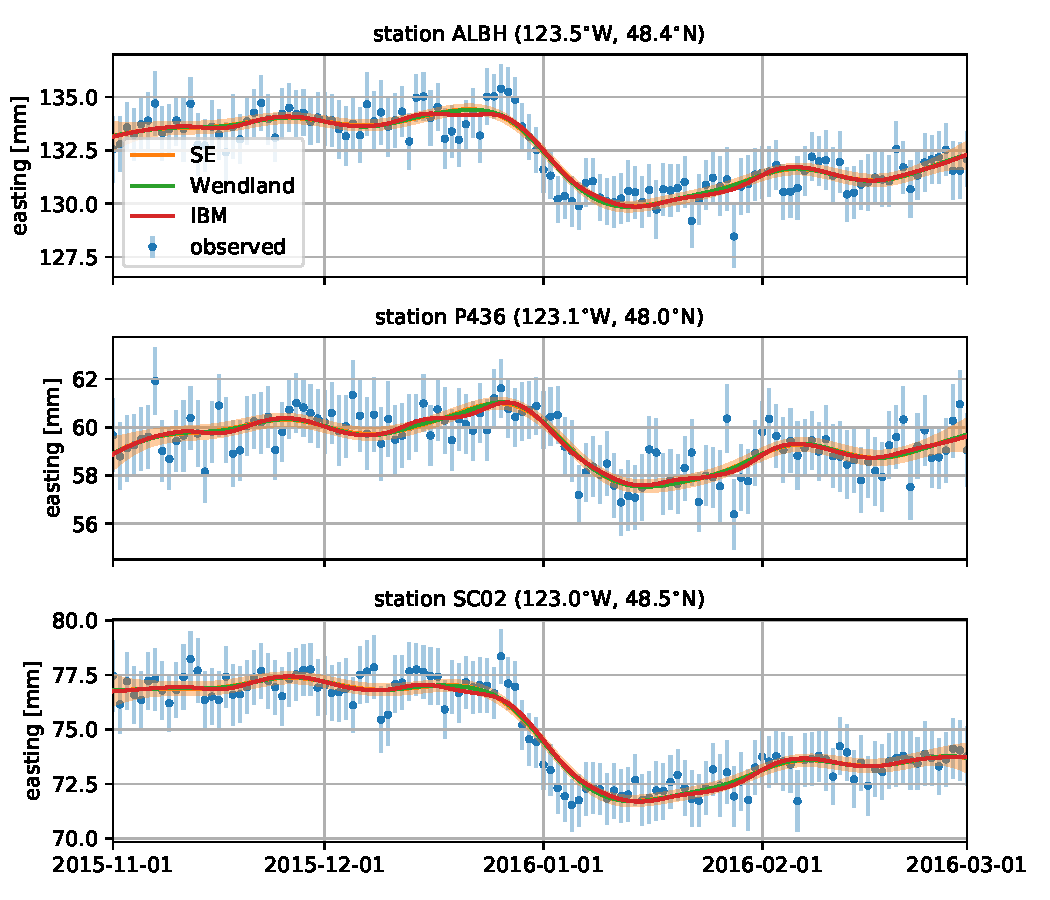
\includegraphics{figures/signal_fit/signal-fit.pdf}
\caption{\DIFdelbeginFL \DIFdelFL{Observed easting }\DIFdelendFL 
\DIFaddbeginFL \DIFaddFL{Easting }\DIFaddendFL component of \DIFaddbeginFL \DIFaddFL{the observed }\DIFaddendFL displacements\DIFdelbeginFL \DIFdelFL{at station P436 }\DIFdelendFL \DIFaddbeginFL \DIFaddFL{, $\data_\e^*$, }\DIFaddendFL and
\DIFdelbeginFL \DIFdelFL{predicted }\DIFdelendFL \DIFaddbeginFL \DIFaddFL{posterior }\DIFaddendFL displacements\DIFaddbeginFL \DIFaddFL{, $\hat{\data}_\e$, during the winter 2015-2016
SSE. We show $\hat{\data}_\e$ for }\DIFaddendFL when \DIFdelbeginFL \DIFdelFL{using different }\DIFdelendFL \DIFaddbeginFL \DIFaddFL{$T_i$ is a SE, Wendland, and
IBM }\DIFaddendFL covariance \DIFdelbeginFL \DIFdelFL{functions for $T$}\DIFdelendFL \DIFaddbeginFL \DIFaddFL{function}\DIFaddendFL . The one standard deviation uncertainties are
shown for \DIFdelbeginFL \DIFdelFL{the observations }\DIFdelendFL \DIFaddbeginFL \DIFaddFL{$\data_\e^*$ }\DIFaddendFL and the \DIFdelbeginFL \DIFdelFL{predicted displacements when using the }\DIFdelendFL \DIFaddbeginFL \DIFaddFL{$\hat{\data}_\e$ that has a }\DIFaddendFL SE
covariance function \DIFaddbeginFL \DIFaddFL{for $T_i$}\DIFaddendFL . For clarity, uncertainties are not
shown for the \DIFaddbeginFL \DIFaddFL{$\hat{\data}_\e$ that have an }\DIFaddendFL IBM \DIFdelbeginFL \DIFdelFL{and }\DIFdelendFL \DIFaddbeginFL \DIFaddFL{or }\DIFaddendFL Wendland covariance
\DIFdelbeginFL \DIFdelFL{functions, but they are nearly equivalent to the uncertainties }\DIFdelendFL \DIFaddbeginFL \DIFaddFL{function for $T_i$. The posterior displacements }\DIFaddendFL for the \DIFdelbeginFL \DIFdelFL{SE }\DIFdelendFL \DIFaddbeginFL \DIFaddFL{different
}\DIFaddendFL covariance \DIFdelbeginFL \DIFdelFL{function}\DIFdelendFL \DIFaddbeginFL \DIFaddFL{functions are all practically indistinguishable}\DIFaddendFL .
}   
\label{fig:Fit}
\end{figure*}

%DIF > % TRANSIENT STRAIN RATES
\subsection{Transient Strain Rates}\label{sec:Results} 
\DIFaddbegin 

%DIF >  Stating how we calculate strain and refering to the figures

\DIFaddend Having established a noise model and a prior for transient
displacements, we \DIFdelbegin \DIFdel{use the cleaned GNSS dataset to }\DIFdelend \DIFaddbegin \DIFadd{can now }\DIFaddend calculate transient strain rates\DIFaddbegin \DIFadd{, $\strain$,
}\DIFaddend in the Puget Sound region \DIFdelbegin \DIFdel{.  We calculate transient strain rates }\DIFdelend \DIFaddbegin \DIFadd{from the GNSS data. We evaluate $\strain$ at
a grid of points spanning the study area }\DIFaddend for each day from January 1,
2010 to May 15, 2017. \DIFdelbegin \DIFdel{The strain rates are estimates at a grid of points spanning the study area. }\DIFdelend In Figure \ref{fig:StrainMap}\DIFdelbegin \DIFdel{we show the transient strain rates }\DIFdelend \DIFaddbegin \DIFadd{, we show a map
view of $\strain$ }\DIFaddend on January 1, 2016, which coincides with the height
of \DIFdelbegin \DIFdel{an SSE. We have included a video showing the }\DIFdelend \DIFaddbegin \DIFadd{the winter 2015-2016 SSE. In Figure \ref{fig:StrainTs}, we show a
time series of $\strain$ at a position on the Olympic Peninsula, which
is where $\strain$ tends to be the largest during SSEs. We also
include a supplementary animation showing a }\DIFaddend map view of \DIFdelbegin \DIFdel{strain rates through timeas supplementary material. The }\DIFdelend \DIFaddbegin \DIFadd{$\strain$ over
time. In each figure, we show the mean and standard deviation of
$\strain$, making it easy to identify which features are statistically
significant.
}

%DIF >  Describe the strain during SSEs and tectonic implications

\DIFadd{The transient }\DIFaddend strain rates shown \DIFaddbegin \DIFadd{for the winter 2015-2016 SSE }\DIFaddend in
Figure \ref{fig:StrainMap} are \DIFdelbegin \DIFdel{generally similar to the strain rates for the other six SSEs considered in this study}\DIFdelend \DIFaddbegin \DIFadd{characteristic of most SSEs in the
Puget Sound region}\DIFaddend . The SSEs cause \DIFaddbegin \DIFadd{trench perpendicular }\DIFaddend compression in
the Olympic Peninsula and extension east of Puget Sound. \DIFdelbegin \DIFdel{For comparison, estimated secular strain rates indicate }\DIFdelend \DIFaddbegin \DIFadd{The strain
transitions from compression to extension around the southern tip of
Vancouver Island, coinciding with where fault slip tends to be
inferred \mbox{%DIFAUXCMD
\citep[e.g.,][]{Dragert2001, Wech2009, Schmidt2010}}%DIFAUXCMD
. Thus,
this pattern of strain is to be expected. Over decadal timescales,
there is }\DIFaddend trench perpendicular compression throughout this study region
\DIFdelbegin \DIFdel{\mbox{%DIFAUXCMD
\citep{Murray2000,McCaffrey2007,McCaffrey2013}}%DIFAUXCMD
. The SSEs are
thus }\DIFdelend \DIFaddbegin \DIFadd{caused by steady tectonic plate motion \mbox{%DIFAUXCMD
\citep{Murray2000,
McCaffrey2007, McCaffrey2013}}%DIFAUXCMD
. When comparing the transient strain
rates caused by SSEs to the secular strain rates, we see that SSEs are
}\DIFaddend concentrating tectonically accumulated strain energy \DIFdelbegin \DIFdel{trench-ward}\DIFdelend \DIFaddbegin \DIFadd{towards the
trench}\DIFaddend , and presumably pushing the subduction zone closer to failure.
\DIFdelbegin \DIFdel{Similar conclusions have been drawn based on fault slip models \mbox{%DIFAUXCMD
\citep[e.g.,][]{Dragert2001,Wech2009,Schmidt2010}}%DIFAUXCMD
, which reveal that SSEs are occurring down-dip of the seismogenic zone and migrating stress upward. A key difference between the strain inferred here and strain that can be derived from fault slip models is that our estimated strain rates are not based on an assumed physical model. In contrast, fault slip models can be biased by errors in the assumed fault geometry or lithospheric rheology. Moreover, the degrees of freedom in fault slip models usually cannot be constrained by GNSS data alone, and it is necessary to impose regularization which further biases the results. Since our estimated strain rates lack such systematic errors, we can be more confident that our solution is unbiased and has meaningful uncertainties.  
}\DIFdelend 

\begin{figure*}
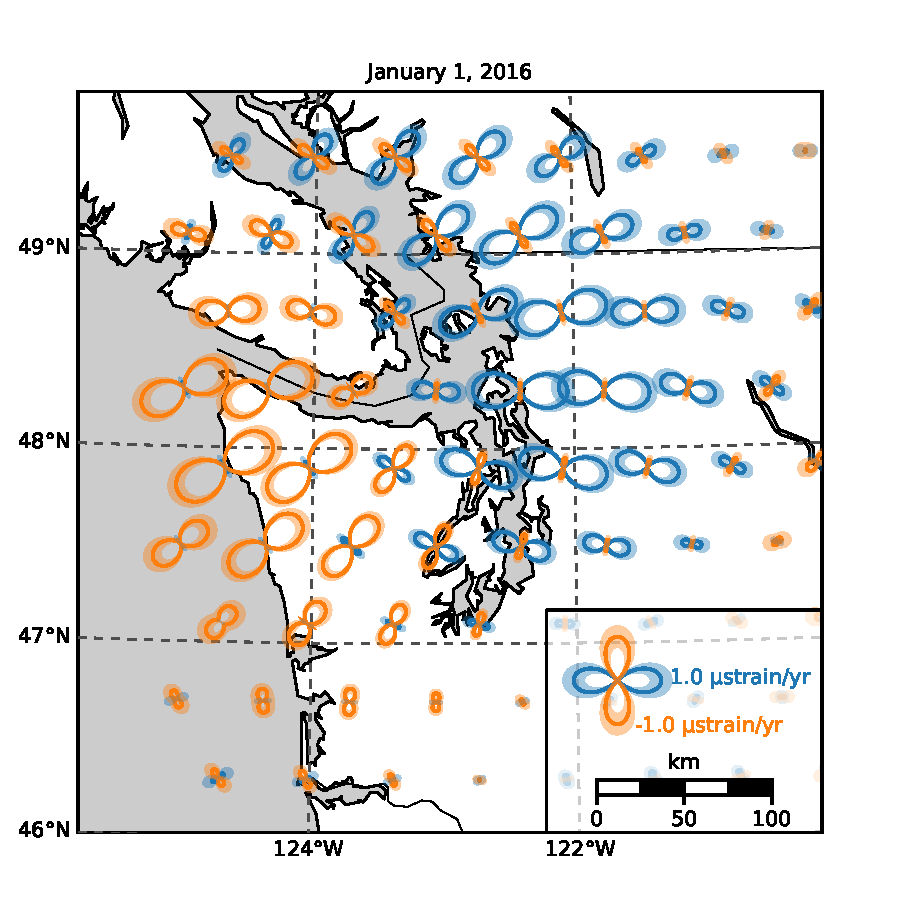
\includegraphics{figures/strain_map/strain-map.pdf}
\caption{\DIFdelbeginFL \DIFdelFL{Estimated transient }\DIFdelendFL 
\DIFaddbeginFL \DIFaddFL{Transient }\DIFaddendFL strain rates during the Winter 2015-2016 SSE. \DIFdelbeginFL \DIFdelFL{Strain }\DIFdelendFL \DIFaddbeginFL \DIFaddFL{The }\DIFaddendFL glyphs
show the normal strain \DIFdelbeginFL \DIFdelFL{rate along each }\DIFdelendFL \DIFaddbeginFL \DIFaddFL{rates as a function of }\DIFaddendFL azimuth, where orange
indicates compression and blue indicates extension. The shaded regions
indicate \DIFaddbeginFL \DIFaddFL{the }\DIFaddendFL one standard deviation uncertainties \DIFdelbeginFL \DIFdelFL{in }\DIFdelendFL \DIFaddbeginFL \DIFaddFL{for }\DIFaddendFL the normal
strain rates.
}   
\label{fig:StrainMap}
\end{figure*}

\DIFdelbegin \DIFdel{In Figure \ref{fig:StrainTs} we show the time dependence of estimated transient strain rates at a position on the Olympic Peninsula, where transient strain rates from SSEs are largest. }\DIFdelend %DIF >  compare seismic tremor to SNR
\DIFaddbegin 

\DIFaddend To verify that the estimated transient strain rates are accurately
identifying geophysical signal, we compare the signal-to-noise ratio
from eq. (\ref{eq:SNR}) \DIFaddbegin \DIFadd{at a point on the Olympic Peninsula }\DIFaddend to the
frequency of seismic tremor (Figure \ref{fig:StrainMag}). A
signal-to-noise ratio greater than ${\sim}3$ can be interpreted as a
detected geophysical signal. \DIFdelbegin \DIFdel{For each detected event there is a corresponding peak }\DIFdelend \DIFaddbegin \DIFadd{We detect nine distinct events, which
each correspond to peaks }\DIFaddend in seismic tremor. \DIFdelbegin \DIFdel{We are also able to clearly identify transient strain associated with a more subtle SSE in August 2014. In between SSEs}\DIFdelend \DIFaddbegin \DIFadd{The smaller events
detected in August 2014 and February 2017 can be considered inter-SSE
events. They were not among the SSEs used to constrain the prior
covariance function. In between peaks in seismic tremor}\DIFaddend , the
signal-to-noise ratio is consistently between 0 and 2, \DIFdelbegin \DIFdel{indicating that
no anomalous non-SSE events are being detected , at least at this location}\DIFdelend \DIFaddbegin \DIFadd{suggesting that
all the transient strain detected at this point on the Olympic
Peninsula is associated with SSEs and inter-SSE events}\DIFaddend .

\begin{figure*}
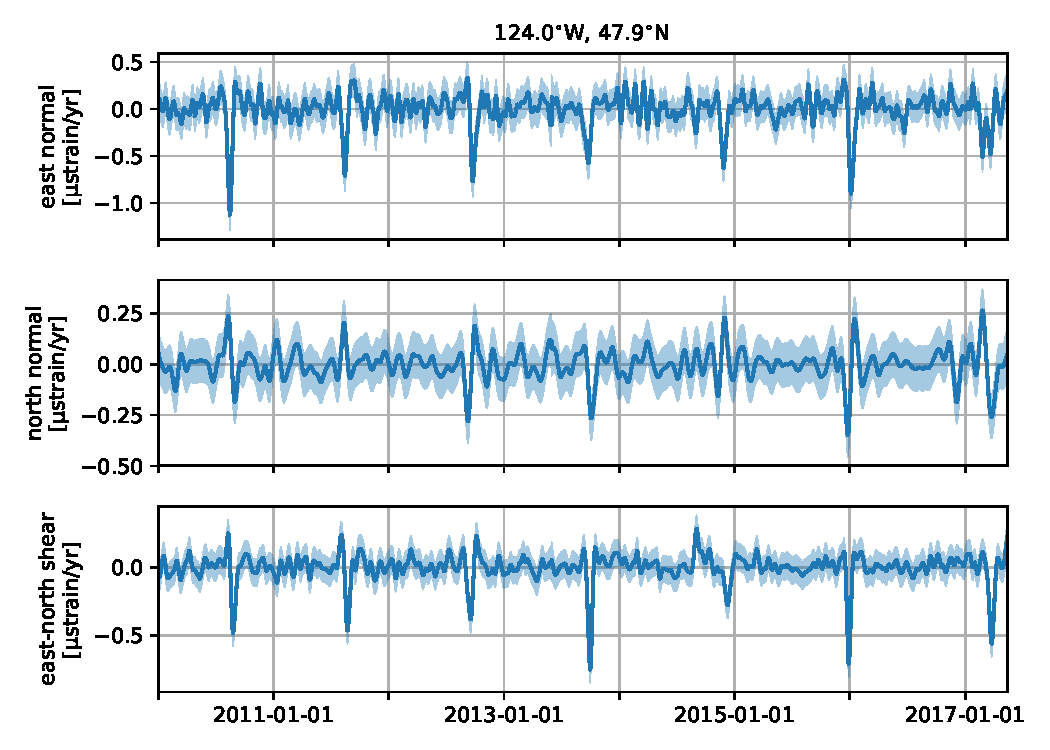
\includegraphics{figures/strain_ts/strain-ts.pdf}
\caption{\DIFdelbeginFL \DIFdelFL{Three components }\DIFdelendFL 
\DIFaddbeginFL \DIFaddFL{Components }\DIFaddendFL of the transient \DIFdelbeginFL \DIFdelFL{horizontal }\DIFdelendFL strain \DIFdelbeginFL \DIFdelFL{rate tensor estimated }\DIFdelendFL \DIFaddbeginFL \DIFaddFL{rates }\DIFaddendFL at the position shown in
Figure \ref{fig:Context}. The shaded regions indicate \DIFaddbeginFL \DIFaddFL{the }\DIFaddendFL one standard
deviation \DIFdelbeginFL \DIFdelFL{uncertainty}\DIFdelendFL \DIFaddbeginFL \DIFaddFL{uncertainties}\DIFaddendFL .
}   
\label{fig:StrainTs}
\end{figure*}

\begin{figure*}
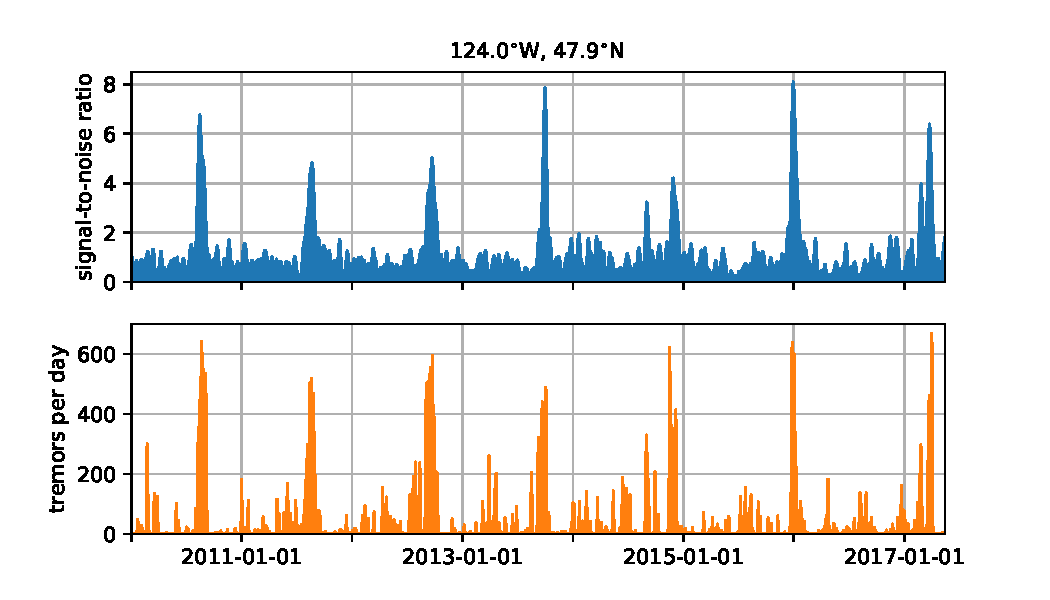
\includegraphics{figures/strain_ts/mag-ts.pdf}
\caption{
(top) Signal-to-noise ratio (eq. \ref{eq:SNR}) at the position shown
in Figure \ref{fig:Context}. (bottom) Frequency of \DIFaddbeginFL \DIFaddFL{seismic }\DIFaddendFL tremors in
the region shown in Figure \ref{fig:Context}.
}   
\label{fig:StrainMag}
\end{figure*}

\DIFdelbegin \section{\DIFdel{Discussion}}%DIFAUXCMD
\addtocounter{section}{-1}%DIFAUXCMD
%DIFDELCMD < %DIFDELCMD < \label{sec:Discussion}%%%
%DIFDELCMD < %%%
\DIFdel{We have demonstrated that transient strain rates estimated with the
method described in Section \ref{sec:Method} can be used to detect SSEs and will be robust to detect other transient geophysical phenomena. Another potential application would be to use GNSS derived transient strain rates to develop noise models for borehole strain meters (BSMs). The Plate Boundary Observatory maintains 43 BSMs in Cascadia, and it has been demonstrated that BSMs are able to record transient geophysical events such as SSEs \mbox{%DIFAUXCMD
\citep[e.g.,][]{Dragert2011}}%DIFAUXCMD
}\DIFdelend %DIF >  note that we are only discussing strain with known origin
\DIFaddbegin 

\DIFadd{The results we have presented indicate that we are identifying the
transient strain that we should expect to see. This is not to say that
there are no unexpected features in $\strain$ that are worth further
exploration}\DIFaddend . However, \DIFdelbegin \DIFdel{noise in BSM data is not well understood, which complicates the use of BSM data for detecting geophysical events. The noise consists, in part, of a long-term decay resulting from the instrument equilibrating with the surrounding rock \mbox{%DIFAUXCMD
\citep{Gladwin1987}}%DIFAUXCMD
. Typically, this noise is dealt with in an ad-hoc manner by fitting and removing exponentials and low-order polynomials. A more rigorous quantification of BSM noise could be performed by analyzing the residuals between the the BSM data and GNSS derived strain rates. }\DIFdelend \DIFaddbegin \DIFadd{a discussion on features in $\strain$ that have
unknown origin would be outside the scope of this paper.
}\DIFaddend 

\DIFdelbegin \DIFdel{There }\DIFdelend %DIF > % DISCUSSION
%DIF > %%%%%%%%%%%%%%%%%%%%%%%%%%%%%%%%%%%%%%%%%%%%%%%%%%%%%%%%%%%%%%%%%%%%
\DIFaddbegin \section{\DIFadd{Discussion}}\label{sec:Discussion}

%DIF > % Areas for improvement and further study
%DIF >  noise model

\DIFadd{Our results demonstrate that GPR is an effective tool for estimating
transient strain rates and detecting geophysical processes from GNSS
data. However, there are some aspects of our method that warrant
further research. For example, there }\DIFaddend is potential for a more thorough
analysis of the spatio-temporal noise in \DIFdelbegin \DIFdel{GNSS data, $\eta$, }\DIFdelend \DIFaddbegin \DIFadd{the GNSS data }\DIFaddend than what was
performed in Section \ref{sec:NoiseModel}. \DIFdelbegin \DIFdel{We }\DIFdelend \DIFaddbegin \DIFadd{Specifically, we }\DIFaddend did not
explore \DIFdelbegin \DIFdel{the spatial covariance of $\eta$. Spatially correlated common mode noise, which results from factors such as reference frame error, is a non-negligible component of GNSS data. We ignore }\DIFdelend \DIFaddbegin \DIFadd{spatially correlated noise, such as }\DIFaddend common mode error\DIFdelbegin \DIFdel{in this study because transients strain rates are insensitive to it. For other geophysical studies based on GNSS data, such as fault slip inversions, it may be necessary to incorporate a spatially covarying noise model \mbox{%DIFAUXCMD
\citep[e.g.,][]{Miyazaki2003}}%DIFAUXCMD
}\DIFdelend \DIFaddbegin \DIFadd{. We
have assumed that any spatially correlated noise has a sufficiently
long wavelength that it has a negligible effect on transient strain
rates}\DIFaddend . We can also improve upon the seasonal \DIFaddbegin \DIFadd{noise }\DIFaddend model used in this
study, which consists of four \DIFdelbegin \DIFdel{spatially uncorrelated }\DIFdelend sinusoids for each station. We did not
explore the \DIFdelbegin \DIFdel{spatial covariance of seasonal deformation or the temporal roughness }\DIFdelend \DIFaddbegin \DIFadd{roughness of the seasonal deformation }\DIFaddend (i.e., the number of
sinusoids needed to describe the \DIFdelbegin \DIFdel{observations}\DIFdelend \DIFaddbegin \DIFadd{deformation}\DIFaddend ). The periodic Gaussian
process \citep{Mackay1998} is an alternative model for seasonal
deformation and is well suited for exploring the roughness of seasonal
deformation.  The periodic Gaussian process has zero mean and the
covariance function
\begin{equation}\label{eq:Periodic}
  T(t,t') = \phi^2 \exp\left(\frac{-\sin(\pi|t - t'|)^2}{2\tau^2}\right). 
\end{equation}
Realizations have annual periodicity and the roughness is controlled
by $\tau$. Decreasing $\tau$ has the same effect as including higher
frequency sinusoids in the seasonal model. The optimal value for
$\tau$ can be found with the REML method\DIFdelbegin \DIFdel{as described in Section \ref{sec:NoiseModel}}\DIFdelend .

%DIF >  issues and potential improvements on numerical consideratiosn
\DIFaddbegin 

%DIF >  Numerical considerations

%DIF >  note that the compact covariance function is not a perfect solution
%DIF >  because it is only compact if the signal has a short timescale. Long
%DIF >  wavelength features will still have a dense covariance matrix. This is
%DIF >  part of the reason why we omitted the temporal noise model.

%DIF >  numerical issues

\DIFadd{Another potential research direction would be to reduce the
computational cost of our method for estimating transient strain
rates. GPR is generally computationally expensive when there are many
observations. }\DIFaddend The transient strain rates estimated in this study are
constrained by \DIFdelbegin \DIFdel{about }\DIFdelend seven years of daily displacement observations from 94
GNSS stations\DIFdelbegin \DIFdel{. It can be computationally intensive to evaluate }\DIFdelend \DIFaddbegin \DIFadd{, which amounts to about 240,000 observations for each
displacement component. For a dataset with this size, it is difficult
to evaluate the matrix inverses in }\DIFaddend eqs. (\ref{eq:PosteriorMean3}) and
(\ref{eq:PosteriorCov3})\DIFdelbegin \DIFdel{for a dataset with this size. We significantly reduce the amount of memory needed to estimate transient strain rates by
describing the temporal covariance of displacements with }\DIFdelend \DIFaddbegin \DIFadd{. We alleviate this computational cost by
using }\DIFaddend a compact Wendland covariance function \DIFdelbegin \DIFdel{. Using }\DIFdelend \DIFaddbegin \DIFadd{for our prior. By using }\DIFaddend a
compact covariance function for our prior\DIFdelbegin \DIFdel{turns }\DIFdelend \DIFaddbegin \DIFadd{, }\DIFaddend eqs.
(\ref{eq:PosteriorMean3}) and (\ref{eq:PosteriorCov3}) \DIFdelbegin \DIFdel{into }\DIFdelend \DIFaddbegin \DIFadd{become }\DIFaddend sparse
systems of equations \DIFdelbegin \DIFdel{, which we then solve with CHOLMOD. CHOLMOD is designed for solving sparse, positive definite systems of equations. The matrix being inverted in eqs. (\ref{eq:PosteriorMean3}) and (\ref{eq:PosteriorCov3}) is not positive definite; however, we can use another partitioned matrix inversion identity from \mbox{%DIFAUXCMD
\citet{Press2007} }%DIFAUXCMD
to partition it into positive definite submatrices to be inverted. Even when using a compact covariance function, it may still be
necessary to reduce the computational burden by dividing the data into subsets and evaluating transient strain rates
for each subset}\DIFdelend \DIFaddbegin \DIFadd{that are more tractable to evaluate. However, the
sparsity decreases when the Wendland covariance function has a larger
time-scale parameter. The Wendland covariance then offers less of a
computational advantage when we were interested in geophysical
processes that occur over longer times-scales. An alternative approach
to dealing with large datasets would be to explore approximation
methods for GPR \mbox{%DIFAUXCMD
\citep[sec. 8]{Rasmussen2006}}%DIFAUXCMD
.
}

%DIF >  additional applications

\DIFadd{In addition to detecting geophysical processes, the GNSS derived
transient strain rates can be used to better understand the data from
borehole strain meters (BSMs). The Plate Boundary Observatory contains
about forty BSMs in the Pacific Northwest, and it has been
demonstrated that BSMs are able to record transient geophysical events
such as SSEs \mbox{%DIFAUXCMD
\citep[e.g.,][]{Dragert2011}}%DIFAUXCMD
. However, there are
complications that prevent BSM data from being used quantitatively in
geophysical studies. One difficulty is that BSM data should be
calibrated with a well known strain source, such as diurnal and
semidiurnal tides \mbox{%DIFAUXCMD
\citep{Hart1996,Roeloffs2010,Hodgkinson2013}}%DIFAUXCMD
.
Unfortunately, the tidal forces at BSMs which record SSEs are strongly
influenced by local bodies of water such as the Straight of Juan de
Fuca, making it difficult to form a theoretical prediction of tidal
strains \mbox{%DIFAUXCMD
\citep{Roeloffs2010}}%DIFAUXCMD
. Another complication is that noise in
BSM data is not well understood. The noise consists, in part, of a
long-term decay resulting from the instrument equilibrating with the
surrounding rock \mbox{%DIFAUXCMD
\citep{Gladwin1987}}%DIFAUXCMD
. Typically, this noise is dealt
with in an ad-hoc manner by fitting and removing exponentials and
low-order polynomials. We envision that the GNSS derived strain rates
from this paper can be used as a reference strain for calibrating BSM
data and quantify its noise}\DIFaddend .


%DIF > % CONCLUSION
%DIF > %%%%%%%%%%%%%%%%%%%%%%%%%%%%%%%%%%%%%%%%%%%%%%%%%%%%%%%%%%%%%%%%%%%%
\section{Conclusion}\label{sec:Conclusion}
\DIFdelbegin \DIFdel{In this paper we }\DIFdelend \DIFaddbegin 

\DIFadd{We }\DIFaddend propose using Gaussian process regression (GPR) to estimate
transient strain rates from GNSS data. Most other methods for
estimating strain rates assume a parametric representation of
deformation, which can bias the results if the parameterization is not
chosen carefully. Here we assume a stochastic, rather than parametric,
prior model for displacements. Our prior model describes how much we
expect transient displacements to covary spatially and temporally. If
we know nothing about the underlying signal that we are trying to
recover, then the prior model can be chosen objectively with maximum
likelihood methods. \DIFdelbegin \DIFdel{Because GPR is a Bayesian method, the uncertainties on our estimated transient strain rates are well quantified, allowing one to discern geophysical signal from noise. }\DIFdelend We demonstrate that GPR is an effective tool for
detecting geophysical \DIFdelbegin \DIFdel{phenomena}\DIFdelend \DIFaddbegin \DIFadd{processes}\DIFaddend , such as slow slip events, in our
application to \DIFdelbegin \DIFdel{GNSS data from Cascadia. One limitation with GPR is that it is not robust against outliers. To overcome this limitation, we have introduced an effective pre-processing method for identifying and removing outliers from GNSS datasets. Another complication with GPR is that it usually involves inverting a dense matrix where the number of rows and columns is equal to the number of observations. This is prohibitive when using several years of daily GNSS observations from a network of several hundred stations. We significantly reduce the computational burden of GPR by using compact Wendland covariance function to describe our prior model}\DIFdelend \DIFaddbegin \DIFadd{the Pacific Northwest}\DIFaddend . While this paper just focuses on
\DIFdelbegin \DIFdel{estimating }\DIFdelend \DIFaddbegin \DIFadd{using GPR to estimate }\DIFaddend transient strain rates \DIFaddbegin \DIFadd{and detect geophysical
processes}\DIFaddend , we believe that GPR is a powerful tool that can be applied
to a wide range of geophysical problems.

%DIF > % ACKNOWLEDGEMENTS
%DIF > %%%%%%%%%%%%%%%%%%%%%%%%%%%%%%%%%%%%%%%%%%%%%%%%%%%%%%%%%%%%%%%%%%%%
\section{Acknowledgements}
This material is based upon work supported by the National Science
Foundation under grant EAR 1245263. The EarthScope Plate Boundary
Observatory data is provided by UNAVCO through the GAGE Facility with
support from the National Science Foundation (NSF) and National
Aeronautics and Space Administration (NASA) under NSF Cooperative
Agreement EAR-1261833. An implementation of the method described in
this paper is named Python-based Geodetic Network Strain software
(PyGeoNS). PyGeoNS is distributed under the MIT License and can be
found at www.github.com/treverhines/PyGeoNS.
\DIFaddbegin 

%DIF > % APPENDIX
%DIF > %%%%%%%%%%%%%%%%%%%%%%%%%%%%%%%%%%%%%%%%%%%%%%%%%%%%%%%%%%%%%%%%%%%%
\appendix
\section{\DIFadd{Outlier detection algorithm}}

\DIFadd{Our outlier detection algorithm is loosely based on the data editing
algorithm from \mbox{%DIFAUXCMD
\citet{Acheson1975}}%DIFAUXCMD
. Let $\data^*$ denote all $n$ GNSS
displacement observations for a single directional component, which
have been made at positions and times $\points$.  We describe
$\data^*$ as a realization of the random vector
}\begin{equation}\DIFadd{\label{eq:OutlierDataVec}
\data = \G\mitbf{m} + v(\points) + \mitbf{w},
}\end{equation}
\DIFadd{where $\G$ and $\mitbf{m}$ are the same as in eq. (\ref{eq:DataVec}),
$v$ is a Gaussian process distributed as $\mathcal{GP}(0,C_v)$, and
$\mitbf{w}$ is a vector of uncorrelated Gaussian noise with known
standard deviations $\mitbf{\sigma} = [\sigma_1, \sigma_2, ...,
\sigma_n]$. The Gaussian process $v$ is intended to describe transient
features in the data that cannot be explained by the linear trend or
seasonal terms in $\G$. We let the temporal covariance of $v$ be a
squared exponential, and we let $v$ be spatially uncorrelated so that,
}\begin{equation}
\DIFadd{C_v(p,p') = \phi^2\exp\left(\frac{-|t - t'|^2}{2\tau^2}\right) \delta_{\pos,\pos'},
}\end{equation}
\DIFadd{where $\delta_{\pos,\pos'} = 1$ if $\pos = \pos'$ and $0$ otherwise.
The spatial covariance of $v$ has little effect on the detected
outliers, and so we have assumed that $v$ is spatially uncorrelated
for simplicity. Based on our experience, $v$ can reasonably describe
most transient features in the data when we set $\phi = 1$ mm and
$\tau = 10$ days.
}

\DIFadd{Our goal is to find the index set of non-outliers in $\data^*$, which
we denote as $\mitbf{\Omega}$. We use a tilde to indicate that an
array only contains elements corresponding to $\mitbf{\Omega}$ (e.g.,
the vector of non-outlier observations is denoted $\tilde{\data}^* =
[d_i^*]_{i \in \mitbf{\Omega}}$). The outliers are identified
iteratively, and we initiate $\mitbf{\Omega}$ with all $n$ indices. We
consider outliers to be data that are poorly explained by the model
$\G\mitbf{m} + v(\points)$, which is determine by the residual vector
}\begin{align}\DIFadd{\label{eq:Residual} 
\mitbf{r} }&\DIFadd{= \data^* - \E{\Big(\G\mitbf{m} + v(\points)\Big) \Big| \Big(\tilde{\data} =
                                                                        \tilde{\data}^*\Big)} }\\
          &\DIFadd{= \data^*  - 
            \left[\begin{array}{cc}
                  C_v(\points,\tilde{\points}) & \G \nonumber \\
                  \end{array}\right]
            \left[\begin{array}{cc}
                  C_v(\tilde{\points},\tilde{\points}) + \mathrm{diag}(\tilde{\mitbf{\sigma}}^2) & \tilde{\G} \\
                  \tilde{\G}^T  & \zeros \\
                  \end{array}\right]^{-1}
            \left[\begin{array}{c}
                  \tilde{\data}^* \\
                  \zeros \\
                  \end{array}\right].
}\end{align}
\DIFadd{Data with abnormally large residuals are identified as outliers. For
each iteration, we compute $\mitbf{r}$ and then update
$\mitbf{\Omega}$ so that it contains the indices of $\mitbf{r}$ whose
weighted values are less than $\lambda$ times the weighted root mean
square of $\tilde{\mitbf{r}}$,
}\begin{equation}\DIFadd{\label{eq:Update}
\mitbf{\Omega} \leftarrow \left\{i : \left|\frac{r_i}{\sigma_i}\right| < \lambda \cdot \sqrt{\frac{1}{|\mitbf{\Omega}|} \sum_{j \in \mitbf{\Omega}} \frac{r_j^2}{\sigma_j^2}} \right\}.
}\end{equation} 
\DIFadd{Iterations continue until the new $\mitbf{\Omega}$ is the same as the
previous $\mitbf{\Omega}$.
}

\DIFadd{The outlier detection algorithm is demonstrated in Figure
\ref{fig:Outliers}. For the demonstration, we use the easting
component of displacements at a single station, SC03, which is located
on Mt. Olympus in Washington state. Station SC03 records anomalous
observations during the winter, presumably because of snow and ice
accumulation, and we want to remove these observations. The station
also records periodic westward motion from slow slip events, and we
want to keep this deformation intact. The detected outliers are shown
in Panel B. For comparison, we also show the detected outliers when we
do not include the Gaussian process $v$ in our model for the data
(Panel A). When $v$ is not included, real transient deformation
resulting from slow slip events is erroneously identified as outliers.
When $v$ is included, the identified outliers only consist of the
anomalous deformation that lacks temporal continuity.  It should be
noted that we use $\lambda = 2.5$ for this demonstration, which causes
the outlier detection algorithm to be particularly aggressive. In
Section \ref{sec:Cascadia}, we clean the data using a more tolerant
$\lambda = 4.0$.
}

\begin{figure*}
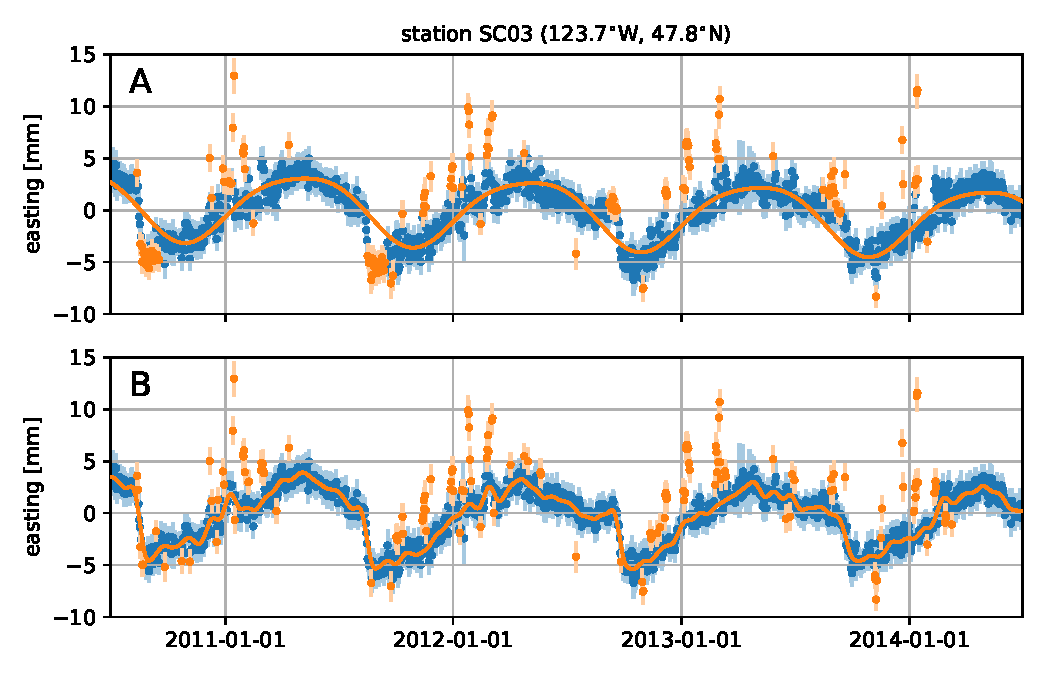
\includegraphics{figures/outliers_new/outliers.pdf}
\caption{
\DIFaddFL{Outliers detected in the easting component of displacements at station
SC03. The orange markers indicate detected outliers. The orange line
is the best fit model to the data, which is used to compute the
residual vector $\mitbf{r}$. The model being fit to the data in Panel
A is $\G\mitbf{m}$, and the model in Panel B is $\G\mitbf{m} +
v(\points)$.
}}
\label{fig:Outliers}
\end{figure*}
\DIFaddend 

\bibliographystyle{gji}
\bibliography{mybib}  

\end{document}
